% Author         : Manuel Lippert
% Version        : 1.1
% Created on     : 11.06.2023
% Last Edited on : 11.06.2023

%%%%%%%%%%%%%%%%%%%%%%%%%%%%%%%%%%%%%%%%%%%%%%%%%%%%%%%%%%%%%%%%%%%%%%%%%%%
%                    !!! Compile with LuaLaTex !!!
%%%%%%%%%%%%%%%%%%%%%%%%%%%%%%%%%%%%%%%%%%%%%%%%%%%%%%%%%%%%%%%%%%%%%%%%%%%

\documentclass[compress,aspectratio=1610,noflama]{beamer}

%--------------------------------------------------------------------------
% Theme
%--------------------------------------------------------------------------

\usepackage{theme/beamerthemefancy}
\usetheme{fancy}

\usepackage{theme/dtklogos} % must be loaded after theme

%--------------------------------------------------------------------------
% Common packages
%--------------------------------------------------------------------------

\usepackage[english]{babel}
\usepackage{graphicx}
\usepackage{multicol}
\usepackage{multimedia}
\usepackage{media9}
\usepackage{hyperref}
\usepackage{tabularx}
\usepackage{tikz}
\usepackage{booktabs}
\usepackage{soul}
%\usepackage[numbers, super]{natbib}
\usepackage{tikz}
\usepackage{multirow}

%--------------------------------------------------------------------------
% Variables
%--------------------------------------------------------------------------

\definecolor{Notablue}{HTML}{3498DB}		%Theoretische Physik
\definecolor{Notared}{HTML}{CF366C}			%Mathematik
\definecolor{Notagreen}{HTML}{19B092}		%Experimentalphysik
\definecolor{Notaorange}{HTML}{FA9D00}		%Chemie/Wahlfach nicht physikalisch
\definecolor{Notagrey}{HTML}{979690}		%Praktikum
\definecolor{Notalavendel}{HTML}{9DBBD8}	%Wahlfächer physikalisch
\definecolor{SPKred}{HTML}{E60005}

\definecolor{codegreen}{rgb}{0,0.6,0}
\definecolor{codegrey}{HTML}{979690}
\definecolor{codepurple}{rgb}{0.58,0,0.82}
\definecolor{codebackground}{gray}{0.92}

\definecolor{Ubtgreen}{RGB}{69, 155, 113}
\usepackage{tikz}
\usetikzlibrary{shapes.geometric, arrows}

\tikzstyle{startstop} = [
    rectangle, rounded corners, 
    minimum width=3cm, 
    minimum height=1cm,
    text centered,  
    align=center,
    fill=Notagreen!30
]

\tikzstyle{error} = [
    rectangle, rounded corners, 
    minimum width=3cm, 
    minimum height=1cm,
    text centered,  
    fill=Notagrey!30
]

\tikzstyle{init} = [
    rectangle, rounded corners, 
    minimum width=3cm, 
    minimum height=1cm, 
    text centered, 
    %draw=black, 
    fill=Notablue!30
]

\tikzstyle{process} = [
    rectangle, rounded corners, 
    minimum width=3cm, 
    minimum height=1cm, 
    text centered, 
    %draw=black, 
    fill=Notaorange!30
]

\tikzstyle{decision} = [
    diamond,
    aspect=3,
    minimum width=2.5cm, 
    minimum height=1.5cm, 
    text centered, 
    %draw=black, 
    fill=Notared!30
]

\tikzstyle{arrow} = [
    thick,
    ->,
    >=stealth
]
\newcommand{\wexb}{\omega_{\mathrm{\:E \times B}}}
\newcommand{\hatwexb}{\widehat{\omega}_{\mathrm{\:E \times B}}}
\newcommand{\exb}{\mathrm{\:E}\times\mathrm{B}}
%\newcommand{\hatwexbampvec}{|\hatwexb|_\mathbf{n}}
\newcommand{\hatwexbamp}{|\hatwexb|_{\nzf}}
%\newcommand{\NR}{N_\mathrm{R}}
%\newcommand{\NB}{N_\mathrm{B}}
\newcommand{\NR}{N_\mathrm{R}}
\newcommand{\NB}{N_\mathrm{B}}
\newcommand{\rlt}{R/L_T}
%\newcommand{\rhoth}{\rho_\mathrm{th}}
\newcommand{\rhoth}{\rho}
\newcommand{\vth}{v_{\mathrm{th}}}
\newcommand{\nzf}{n_\mathrm{ZF}}
\newcommand{\kzf}{k_\mathrm{ZF}}
\newcommand{\xcoord}{x}
\newcommand{\ycoord}{y}

\newcommand{\Ns}{N_\mathrm{s}}
\newcommand{\Nvpar}{N_{\nu_\parallel}}
\newcommand{\Nmu}{N_\mu}
\usepackage{tikz}

\usetikzlibrary{mindmap,backgrounds}
\usetikzlibrary{decorations.pathmorphing}
\usetikzlibrary{decorations.markings}
\usetikzlibrary{arrows.meta,bending}

%--------------------------------------------------------------------------
% Variables
%--------------------------------------------------------------------------

\newcommand{\backgroundpicture}{Comparison/Boxsize/S6_rlt6.0_boxsize1-2-3-4x1_Ns16_Nvpar48_Nmu9_wexb_comparison.pdf}
\newcommand{\backgroundxshift}{0.27\paperwidth}
\newcommand{\backgroundwidth}{0.7\paperwidth} 

\newcommand{\logopicture}{Uni_Logo_white_black}

%--------------------------------------------------------------------------
% Functions, Graphics, Tikz, Underlines
%--------------------------------------------------------------------------

\graphicspath{{../pictures/}}

\newcommand{\vect}[1]{\boldsymbol{\mathbf{#1}}}

\setul{0.3ex}{0.2ex}

\makeatletter 
\let\UL\ul 
\renewcommand\ul{
	\let\set@color\beamerorig@set@color 
	\let\reset@color\beamerorig@reset@color 
	\UL} 
\makeatother

%--------------------------------------------------------------------------
% Document
%--------------------------------------------------------------------------

\title{Size Convergence of the E$\times$B \\ Staircase Pattern in Flux Tube \\ Simulations of Ion
Temperature \\ Gradient-Driven Turbulence}
\subtitle{~}
\author{Manuel Lippert}
\institute{Theoretical Physics V}

\begin{document}

	\maketitle

	%\begin{frame}{Gliederung}
	%	\tableofcontents[hideallsubsections]
	%\end{frame}

	\section*{Motivation}
	\begin{frame}
		\frametitle{Motivation}

		\begin{center}
			\begin{itemize}
				\item <2-> Ion temperature gradient-driven turbulence close to marginal stability exhibits Zonal flow pattern formation on mesoscales 
				\item <3-> Patterns are called $\exb$ staircase structures
			\end{itemize}
		\end{center}
		\bigskip
		\onslide<4-> Observed pattern formation in
		\begin{center}
			\begin{itemize}
				\item <5-> local gradient-driven flux-tube simulations, including collisions and background $\exb$ shear,
				\item <6-> local flux-driven realizations, including mean electric field shear,
				\item <7-> global gradient-driven and global flux-driven studies.
			\end{itemize}
			\bigskip
			\onslide<8-> \textbf{Does the basic pattern size always converges to the box size, or is there a typical mesoscale size inherent to staircase structures also in a local flux-tube description?}
		\end{center}
	\end{frame}

	\section*{Theory}

	\begin{frame}
		\frametitle{Charged Particle Motion}

		\begin{center}
			\begin{tabular}{>{\onslide<2->}c<{\onslide}@{\hspace{0.5cm}} >{\onslide<3->}c<{\onslide}@{\hspace{0.5cm}} >{\onslide<4->}c<{\onslide}}
				\textbf{Lorentz force} & 
				\textbf{Electric force} & 
				\textbf{Inhomogeneous magnetic field} \\
				$F_{\perp, B} = |q| v_\perp B$ & 
				$F_{\parallel,E} = qE_\parallel$ & 
				$F_{\parallel,\nabla_{\!\parallel} B} = - \underbrace{\frac{mv^2_{\perp}}{2B}}_{\mu} \nabla_{\!\parallel} B$ \\
				% \usetikzlibrary{mindmap,backgrounds}
% \usetikzlibrary{decorations.pathmorphing}
% \usetikzlibrary{decorations.markings}
% \usetikzlibrary{arrows.meta,bending}

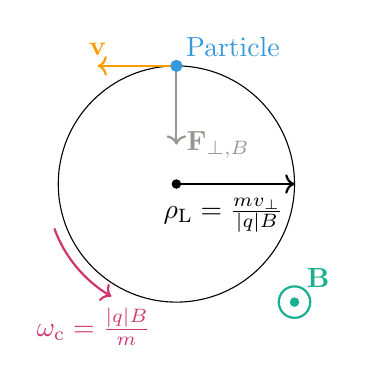
\begin{tikzpicture}
    % Circle
    \draw (0,0) circle (1.5);
    \filldraw (0,0) circle (1.5pt);
    % Force
    \draw[thick, Notagrey, <-] (90:0.5) node[right, Notagrey]{$\vect{F}_{\perp, B}$} -- ++ (90:1.0) node[coordinate] (x) {};
    % Larmor radius
    \draw[thick, black, ->] (0,0) -- ++(0:1.5);
    \draw (0.6,-0.4) node {$\rho_\mathrm{L} = \frac{mv_{\perp}}{|q|B}$};
    % Velocity
    \draw[thick,Notaorange, ->] (x) -- ++(180:1cm) node[above, Notaorange]{$\vect{v}$};
    % Cyclontron freqency
    \draw[thick, ->, Notared] (200:1.1*1.5) arc(200:240:1.1*1.5);
    \draw (240:1.4*1.5) node[Notared] {$\omega_\mathrm{c} = \frac{|q|B}{m}$};
    % Particle
    \filldraw [Notablue] (x) circle (2pt);
    \draw (x) node[above right, Notablue]{Particle};
    % Magnetic field
    \draw [thick, Notagreen] (1.5,-1.5) circle (0.2);
    \filldraw [Notagreen] (1.5,-1.5) circle (1.5pt);
    \draw (1.8,-1.2) node[Notagreen]{$\vect{B}$};
\end{tikzpicture} & 
				% \usetikzlibrary{mindmap,backgrounds}
% \usetikzlibrary{decorations.pathmorphing}
% \usetikzlibrary{decorations.markings}
% \usetikzlibrary{arrows.meta,bending}

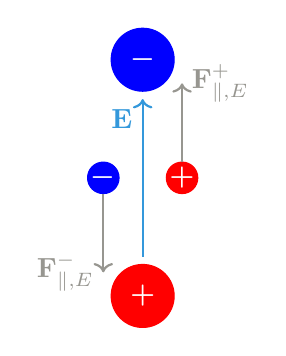
\begin{tikzpicture}
    % Charge
    \draw [fill=blue, blue] (0,1.5) circle (0.4) node[white, font=\boldmath]{$-$};
    \draw [fill=red, red] (0,-1.5) circle (0.4) node[white, font=\boldmath]{$+$};
    \draw [fill=blue, blue] (-0.5,0) circle (0.2) node[white, font=\boldmath]{$-$};
    \draw [fill=red, red] (0.5,0) circle (0.2) node[white, font=\boldmath]{$+$};
    % Electric field
    \draw[thick,Notablue, ->] (0,-1) -- (0,1) node[below left, Notablue] {$\vect{E}$};
    % Force
    \draw[thick, Notagrey, ->] (-0.5, -0.2) -- (-0.5, -1.2);
    \draw (-0.5, -1.2) node[left, Notagrey]{$\vect{F}^{-}_{\parallel,E}$};
    \draw[thick, Notagrey, ->] (0.5, 0.2) -- (0.5, 1.2);
    \draw (0.5, 1.2) node[right, Notagrey]{$\vect{F}^{+}_{\parallel,E}$};
\end{tikzpicture} & 
				% \usetikzlibrary{mindmap,backgrounds}
% \usetikzlibrary{decorations.pathmorphing}
% \usetikzlibrary{decorations.markings}
% \usetikzlibrary{arrows.meta,bending}

{
\def\ang{36}
\def\Rx{0.7}
\def\Ry{1.14}
\def\h{0.5}
\def\H{3}
\def\W{4}
\def\NB{2}

\begin{tikzpicture}

	\coordinate (O) at (0,0);
	\coordinate (N) at (0,0.24*\H);
	\coordinate (M) at (0,0.45*\H);
	\coordinate (B) at (\ang:\H);

	% Magnetic momentum (1/2)
	\draw [thick, Notared] (0,\Ry) arc (90:270:{\Rx} and {\Ry});
	% Magnetic field
	\foreach \i [evaluate={\y=(0.34*\H)*\i^2/\NB; \out=1*\i^2; \in=180+10*\i^2; \f=0.80-0.10*\i;}] in {1,...,\NB}{
	  \draw [thick, Notagreen, <-] (-0.95*\H, 0.7*\y/\H) to[out= \out,in= \in,looseness=0.8] (0.25*\W, \y);
	  \draw [thick, Notagreen, <-] (-0.95*\H,-0.7*\y/\H) to[out=-\out,in=-\in,looseness=0.8] (0.25*\W,-\y);
	}
	\node [Notagreen] at (0.26*\W,0.52*\H) {$\vect{B}$};
	% Force
	\draw [thick, Notagrey, ->] ( 95:{\Rx} and {\Ry}) --++ (-25:0.8*\Ry) node[right=0, Notagrey] {$\vect{F}_{\parallel,\nabla_{\!\parallel} B}$};
	\draw [thick, Notagrey, ->] (-95:{\Rx} and {\Ry}) --++ ( 25:0.8*\Ry) node[right=1, Notagrey] {$\vect{F}_{\parallel,\nabla_{\!\parallel} B}$};
	% Magnetic momentum (2/2)
	\draw [thick, Notared] (0,\Ry) arc (90:-90:{\Rx} and {\Ry});
	\draw [thick, Notared, ->] (0,0) --++ (-0.3*\W,0) node[left, Notared] {$\vect{\mu}$};
	% Particle
	\filldraw [Notablue] (-95:{\Rx} and {\Ry}) circle (2pt);
	\filldraw [Notablue] ( 95:{\Rx} and {\Ry}) circle (2pt);
	\draw (-3,1) node[above right, Notablue]{Particle};

\end{tikzpicture}} \\
			\end{tabular}
		\end{center}
	\end{frame}
	
	\begin{frame}
		\frametitle{Drift in the Gyrocenter}
		\begin{center}
			\begin{tabular}{>{\onslide<2->}c<{\onslide} >{\onslide<3->}c<{\onslide} >{\onslide<3->}c<{\onslide}}
				{\boldmath $\exb$} \textbf{Drift} & 
				{\boldmath $\nabla B$} \textbf{Drift} & 
				\textbf{Curvature Drift} \\
				$\vect{v}_{E} = \frac{\vect{E}\times\vect{B}}{B^2}$ & 
				$\vect{v}_{\nabla B} = \frac{m v^2_{\perp}}{2 q}\frac{\vect{B}\times \nabla B}{B^3}$ & 
				$\vect{v}_{\kappa} = \frac{m v^2_{\parallel}}{qB^2}\vect{B}\times \underbrace{\vect{\kappa}}_{\frac{\nabla B}{B}} = \frac{m v^2_{\parallel}}{q} \frac{\vect{B}\times \nabla B}{B^3}$\\[1cm]
				% \usetikzlibrary{mindmap,backgrounds}
% \usetikzlibrary{decorations.pathmorphing}
% \usetikzlibrary{decorations.markings}
% \usetikzlibrary{arrows.meta,bending}

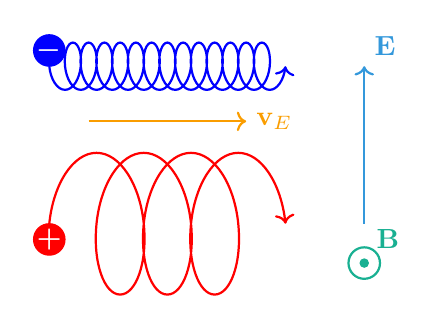
\begin{tikzpicture}
    % Electron
    \draw[thick,decoration={segment length=2mm, amplitude=0.3cm, coil},decorate,<-,blue] (3,0) -- (0,0);
    \draw [fill=blue, blue] (0,0.2) circle (0.2) node[white, font=\boldmath]{$-$};
    % Ion
    \draw[thick,decoration={coil, aspect = -0.5, amplitude = -0.9cm, segment length=6mm},decorate,<-,red] (3,-2) -- (0,-2);
    \draw [fill=red, red] (0,-2.2) circle (0.2) node[white, font=\boldmath]{$+$};
    % Electric field
    \draw[thick,Notablue, ->] (4,-2) -- (4,0) node[above right, Notablue]{$\vect{E}$};
    % Drift velocity
    \draw[thick,Notaorange, ->] (0.5,-0.7) -- (2.5,-0.7) node[right, Notaorange]{$\vect{v}_{E}$};
    % Magnetic field
    \draw [thick, Notagreen] (4,-2.5) circle (0.2);
    \filldraw [Notagreen] (4,-2.5) circle (1.5pt);
    \draw (4.3,-2.2) node[Notagreen]{$\vect{B}$};
\end{tikzpicture} & 
				\multicolumn{2}{>{\onslide<3->}c<{\onslide}}{% \usetikzlibrary{mindmap,backgrounds}
% \usetikzlibrary{decorations.pathmorphing}
% \usetikzlibrary{decorations.markings}
% \usetikzlibrary{arrows.meta,bending}

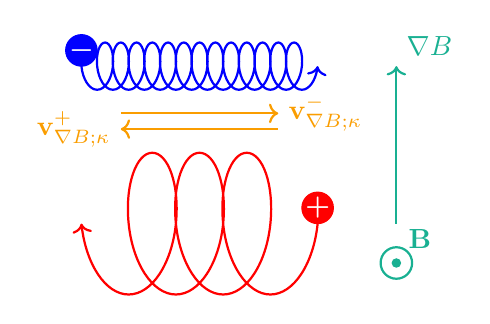
\begin{tikzpicture}
    % Electron
    \draw[thick,decoration={segment length=2mm, amplitude=0.3cm, coil},decorate,<-,blue] (3,0) -- (0,0);
    \draw [fill=blue, blue] (0,0.2) circle (0.2) node[white, font=\boldmath]{$-$};
    % Ion
    \draw[thick,decoration={coil, aspect = -0.5, amplitude = -0.9cm, segment length=6mm},decorate,<-,red] (0,-2) -- (3,-2);
    \draw [fill=red, red] (3,-1.8) circle (0.2) node[white, font=\boldmath]{$+$};
    % Grad B field
    \draw[thick,Notagreen, ->] (4,-2) -- (4,0) node[above right, Notagreen]{$\nabla B$};
    % Drift velocity
    \draw[thick,Notaorange, ->] (0.5,-0.6) -- (2.5,-0.6) node[right, Notaorange]{$\vect{v}^{-}_{\nabla B;\kappa}$};
    \draw[thick,Notaorange, <-] (0.5,-0.8) node[left, Notaorange]{$\vect{v}^{+}_{\nabla B;\kappa}$} -- (2.5,-0.8);
    % Magnetic field
    \draw [thick, Notagreen] (4,-2.5) circle (0.2);
    \filldraw [Notagreen] (4,-2.5) circle (1.5pt);
    \draw (4.3,-2.2) node[Notagreen]{$\vect{B}$};
\end{tikzpicture}} \\
			\end{tabular}
		\end{center}
	
	\end{frame}
	\begin{frame}
		\frametitle{Magnetic Confinement in Tokamak}
		\begin{center}
			\begin{tabular}{>{\onslide<2->}c<{\onslide} >{\onslide<2->}c<{\onslide}}
				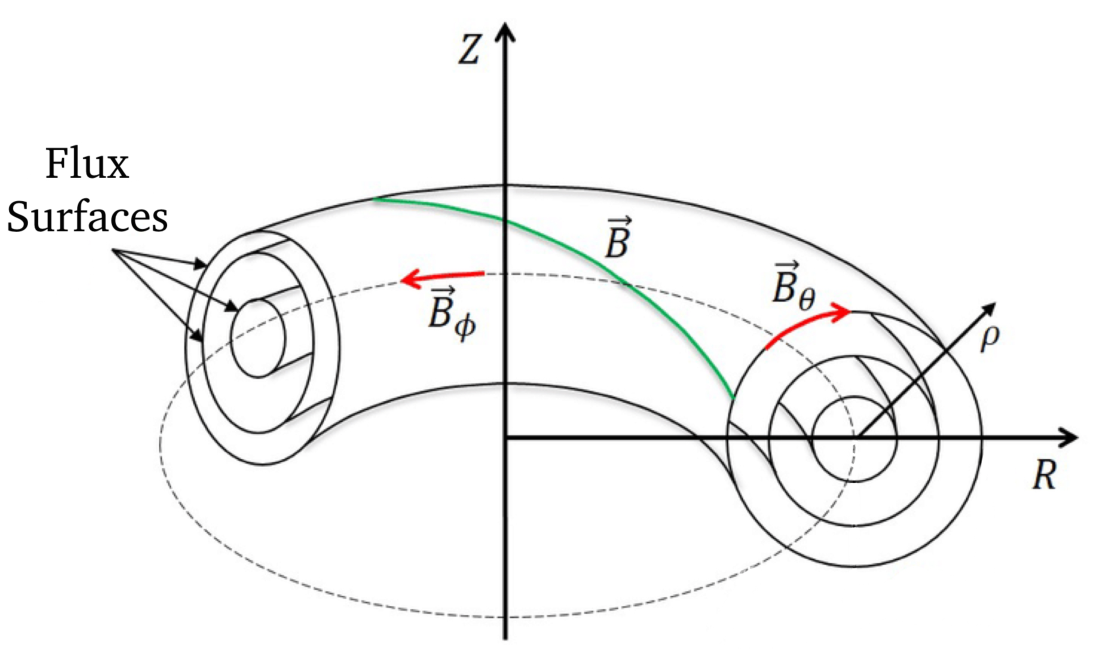
\includegraphics[width=0.6\paperwidth]{Theory/Tokamak-Torus.pdf} & $\beta = \frac{nT}{\mu_0 B^2/2}$
			\end{tabular}
		\end{center}
	\end{frame}

	\begin{frame}
		\frametitle{Ion Temperature Gradient (ITG)-driven Instability}
		\begin{center}
			\onslide<2->% \usetikzlibrary{mindmap,backgrounds}
% \usetikzlibrary{decorations.pathmorphing}
% \usetikzlibrary{decorations.markings}
% \usetikzlibrary{arrows.meta,bending}

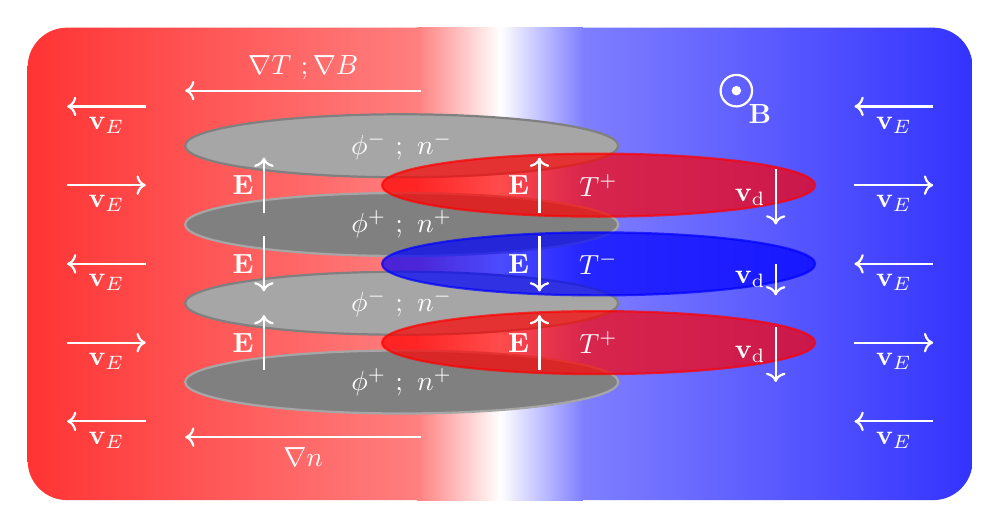
\begin{tikzpicture}

    % Temperature background
    % \shade [left color=red, right color= white, rounded corners = 0cm] (0,0) rectangle (6,6);
    % \shade [left color=white, right color= blue, rounded corners = 0cm] (6,0) rectangle (12,6);

    \onslide<2->{
    \shade [left color=red!80!white, right color= red!50!white]  (5,0) {[rounded corners=0.5cm] --++ (-5,0)  --++ (0,6)} --++ (5,0)  -- cycle;
    \shade [left color=red!50!white, right color= white] (4.95,0) --++ (1.05,0)  --++ (0,6) --++ (-1.05,0)  -- cycle;

    \shade [left color=blue!50!white, right color= blue!80!white]  (7,0) {[rounded corners=0.5cm] --++ (5,0)  --++ (0,6)} --++ (-5,0)  -- cycle;
    \shade [left color=white, right color= blue!50!white] (6,0) --++ (1.05,0)  --++ (0,6) --++ (-1.05,0)  -- cycle;

    }

    \onslide<7->{
    % Density and Potencial cells
    \draw [thick, gray, opacity=1, fill = gray!70!white] (4.75,4.5) ellipse (2.75 and 0.4) node[white, opacity=1]{$\phi^{-}~;~n^{-}$};
    \draw [thick, gray!70!white, opacity=1, fill = gray] (4.75,3.5) ellipse (2.75 and 0.4) node[white, opacity=1]{$\phi^{+}~;~n^{+}$};
    \draw [thick, gray, opacity=1, fill = gray!70!white] (4.75,2.5) ellipse (2.75 and 0.4) node[white, opacity=1]{$\phi^{-}~;~n^{-}$};
    \draw [thick, gray!70!white, opacity=1, fill = gray] (4.75,1.5) ellipse (2.75 and 0.4) node[white, opacity=1]{$\phi^{+}~;~n^{+}$};
    }

    \onslide<4->{
    % Temperature cells
    \draw [thick, red, opacity=0.7, fill = red]   (7.25,4) ellipse (2.75 and 0.4) node[white, opacity=1]{$T^{+}$};
    \draw [thick, blue, opacity=0.7, fill = blue] (7.25,3) ellipse (2.75 and 0.4) node[white, opacity=1]{$T^{-}$};
    \draw [thick, red, opacity=0.7, fill = red]   (7.25,2) ellipse (2.75 and 0.4) node[white, opacity=1]{$T^{+}$};
    }

    \onslide<3->{
    % Temperature and magnetic field gradient
    \draw[thick, white, <-] (2,5.2) -- (5,5.2) node[midway, above, white]{$\nabla T~;\nabla B$};

    % Magnetic field
    \draw [thick, white] (9,5.2) circle (0.2);
    \filldraw [white] (9,5.2) circle (1.5pt);
    \draw (9.3,4.9) node[white]{$\vect{B}$};
    }

    \onslide<6->{
    % Density gradient
    \draw[thick, white, <-] (2,0.8) -- (5,0.8) node[midway, below, white]{$\nabla n$};
    }

    \onslide<8->{
    % Electric field
    \draw[thick, white, <-] (3,4.35) -- (3,3.65) node[midway, below, left]{$\vect{E}$};
    \draw[thick, white, <-] (6.5,4.35) -- (6.5,3.65) node[midway, below, left]{$\vect{E}$};
    \draw[thick, white, ->] (3,3.35) -- (3,2.65) node[midway, below, left]{$\vect{E}$};
    \draw[thick, white, ->] (6.5,3.35) -- (6.5,2.65) node[midway, below, left]{$\vect{E}$};
    \draw[thick, white, <-] (3,2.35) -- (3,1.65) node[midway, below, left]{$\vect{E}$};
    \draw[thick, white, <-] (6.5,2.35) -- (6.5,1.65) node[midway, below, left]{$\vect{E}$};
    }

    \onslide<5->{
    % Grad B and curvature drift velocity
    \draw[thick, white, ->] (9.5,4.2) -- (9.5,3.5) node[midway, left, white]{$\vect{v}_\mathrm{d}$};
    \draw[thick, white, ->] (9.5,3)   -- (9.5,2.6) node[midway, left, white]{$\vect{v}_\mathrm{d}$};
    \draw[thick, white, ->] (9.5,2.2) -- (9.5,1.5) node[midway, left, white]{$\vect{v}_\mathrm{d}$};
    }

    \onslide<9->{
    % ExB drift velocity
    \draw[thick, white, <-] (10.5,5) -- (11.5,5) node[midway, below, white]{$\vect{v}_{E}$};
    \draw[thick, white, ->] (10.5,4) -- (11.5,4) node[midway, below, white]{$\vect{v}_{E}$};
    \draw[thick, white, <-] (10.5,3) -- (11.5,3) node[midway, below, white]{$\vect{v}_{E}$};
    \draw[thick, white, ->] (10.5,2) -- (11.5,2) node[midway, below, white]{$\vect{v}_{E}$};
    \draw[thick, white, <-] (10.5,1) -- (11.5,1) node[midway, below, white]{$\vect{v}_{E}$};
    \draw[thick, white, <-] (0.5,5)  --  (1.5,5) node[midway, below, white]{$\vect{v}_{E}$};
    \draw[thick, white, ->] (0.5,4)  --  (1.5,4) node[midway, below, white]{$\vect{v}_{E}$};
    \draw[thick, white, <-] (0.5,3)  --  (1.5,3) node[midway, below, white]{$\vect{v}_{E}$};
    \draw[thick, white, ->] (0.5,2)  --  (1.5,2) node[midway, below, white]{$\vect{v}_{E}$};
    \draw[thick, white, <-] (0.5,1)  --  (1.5,1) node[midway, below, white]{$\vect{v}_{E}$};
    }

\end{tikzpicture}
		\end{center}
	\end{frame}


	\begin{frame}
		\frametitle{Zonal Flows}
		\begin{center}
			\onslide<2->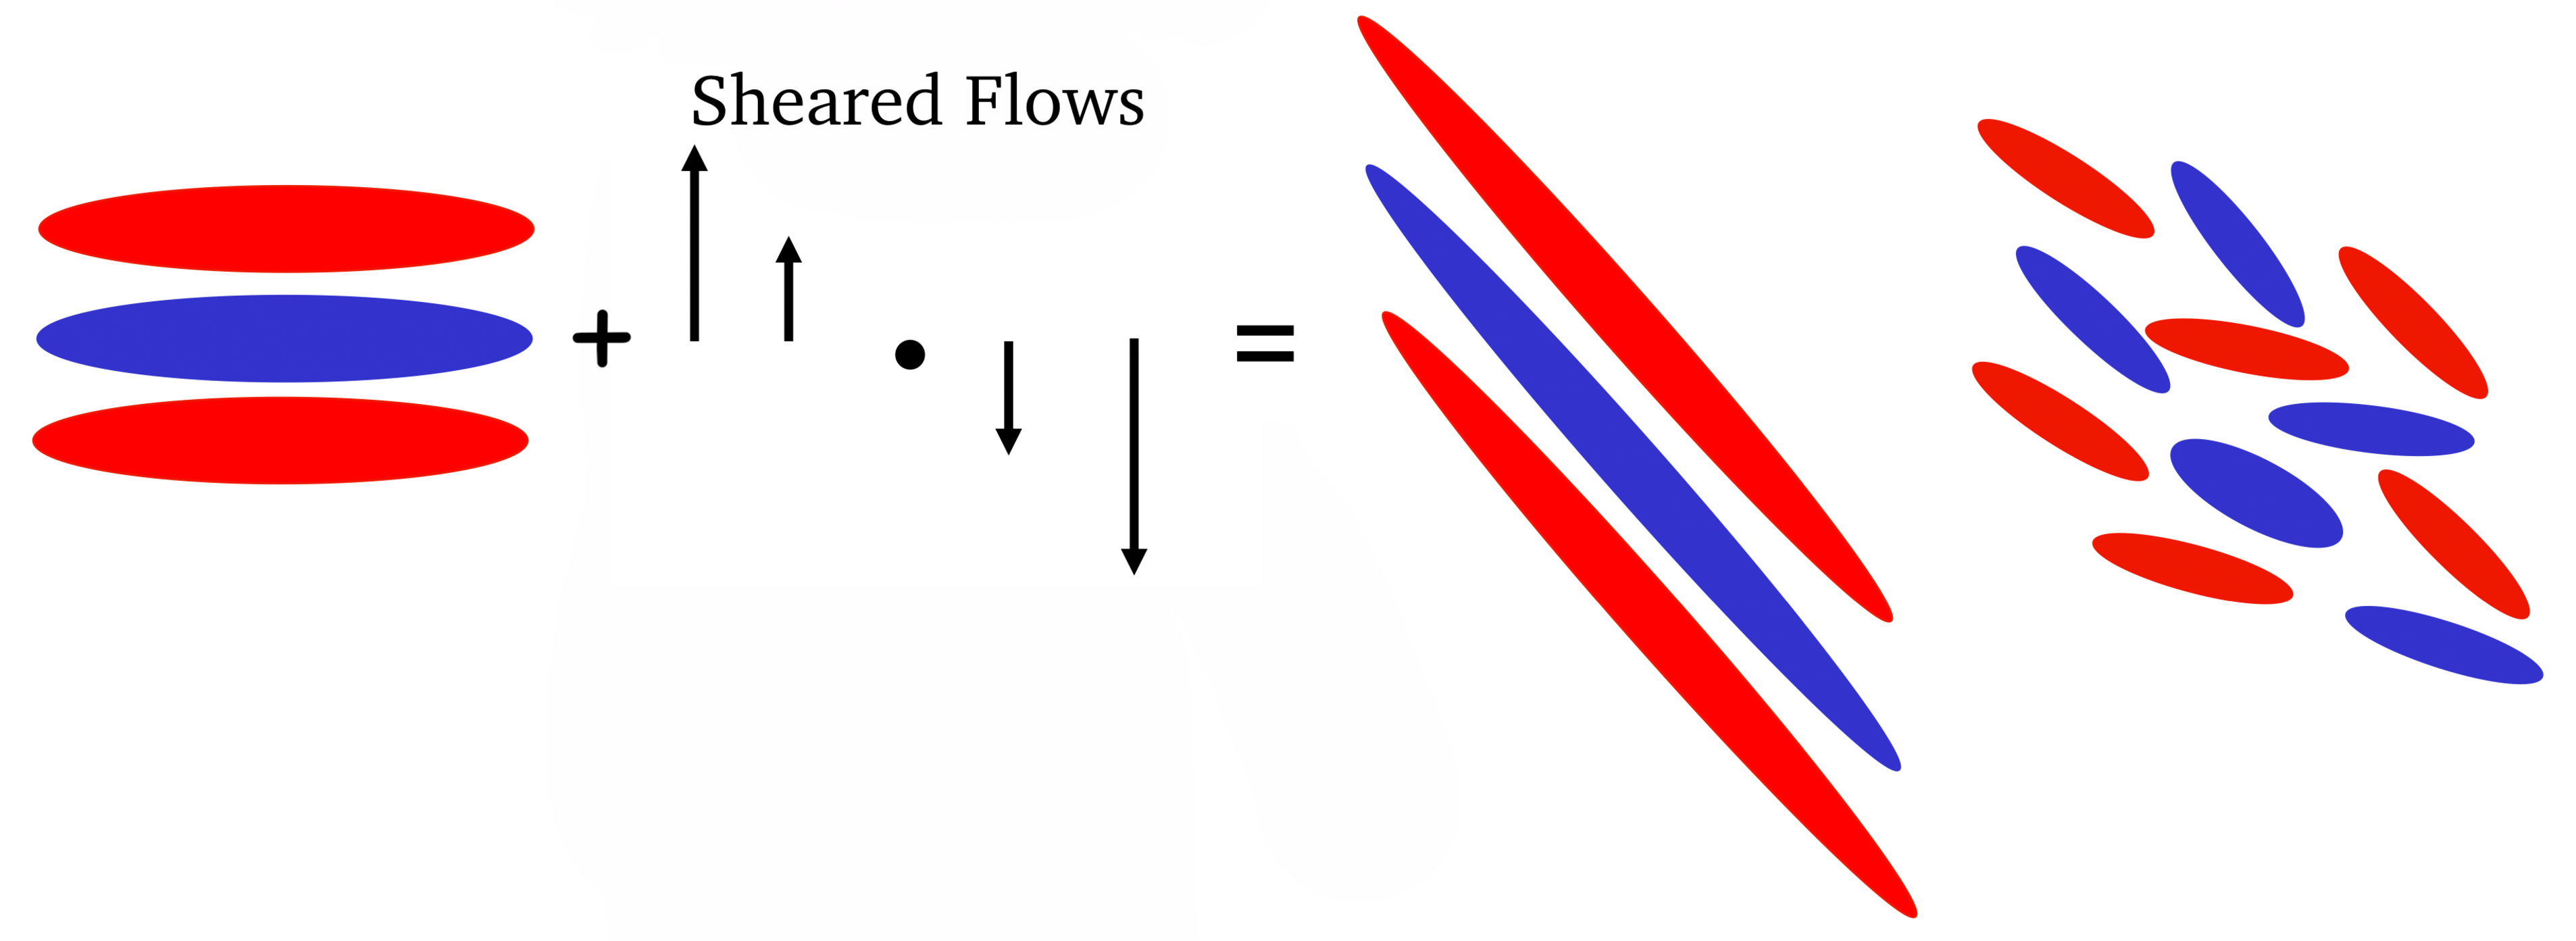
\includegraphics[width = 0.8\paperwidth]{Theory/Zonal-Flow-Generation.pdf}
			%\begin{itemize}
			%	\item <3-> Zonal flows are linked to the $\exb$ flows
			%	\item <4-> Zonal flow is tangential to the flux-surfaces and does not contribute to the turbulent transport across the flux-surfaces
			%\end{itemize}
		\end{center}
	\end{frame}

	\begin{frame}
		\frametitle{Shearing Rate}

		\onslide<2-> Pattern formation occurs in the stabilized tokamak plasma the so-called $\exb$ staircase structure. \\\bigskip
		
		\onslide<3-> Properties:
		\begin{enumerate}
			\item[(1)] <4-> They occur on a \textit{radial mesoscale} of order of $\rho_\mathrm{L} < 10\,\rhoth < R$
			\item[(2)] <5-> The structure are \textit{quasi stationary} in space and vary on time scales much longer than the typical turbulence time scales.
			\item[(3)] <6-> They have a \textit{typical amplitude} of the order of $10^{-1} \vth/R$.
			\item[(4)] <7-> Turbulent transport occurs in \textit{avalanches} with propagation strongly linked to the local $\exb$ shearing rate.
		\end{enumerate}
		\onslide<8->{
		\begin{center}
			\begin{tabular}{c c}
				$\wexb = \frac{1}{2} \frac{\partial^2 \langle \phi \rangle}{\partial \xcoord^2}$ & $\langle \phi \rangle = \frac{1}{L_\ycoord} \int_0^{L_\ycoord} \mathrm{d}\ycoord ~ \phi(\xcoord,\ycoord,s=0)$ \\
			\end{tabular}
		\end{center}
		}
	\end{frame}

	%\begin{frame}
	%	\frametitle{Vlasov Equation}
	%	\begin{gather*}
	%		\frac{\partial f}{\partial t} + \frac{\partial f}{\partial \vect{x}} \cdot \frac{\mathrm{d}\vect{x}}{\mathrm{d}t} + \frac{\partial f}{\partial \vect{v}} \cdot \frac{\mathrm{d}\vect{v}}{\mathrm{d}t} = 0
	%	\end{gather*}
	%	\begin{gather*}
	%		n = \int \mathrm{d}\vect{v}\,f(\vect{x}, \vect{v}, t) \qquad j = q \int \mathrm{d}\vect{v}\, v f(\vect{x}, \vect{v}, t)
	%	\end{gather*}
	%	\begin{gather*}
	%		\begin{aligned}
	%			\nabla \cdot \vect{B} &= 0 &\qquad \nabla \times \vect{B} &= \mu_0\left( \sum_\mathrm{species} j + \epsilon_0 \frac{\partial \vect{E}}{\partial t} \right) \\
	%			\nabla \cdot \vect{E} &= \frac{1}{\epsilon_0} \sum_\mathrm{species} qn &\qquad \nabla \times \vect{E} &= - \frac{\partial \vect{B}}{\partial t}
	%		\end{aligned}
	%	\end{gather*}
	%\end{frame}

	\begin{frame}
		\frametitle{Gyrokinetics}
		
		\only<4>{
			\begin{center}
				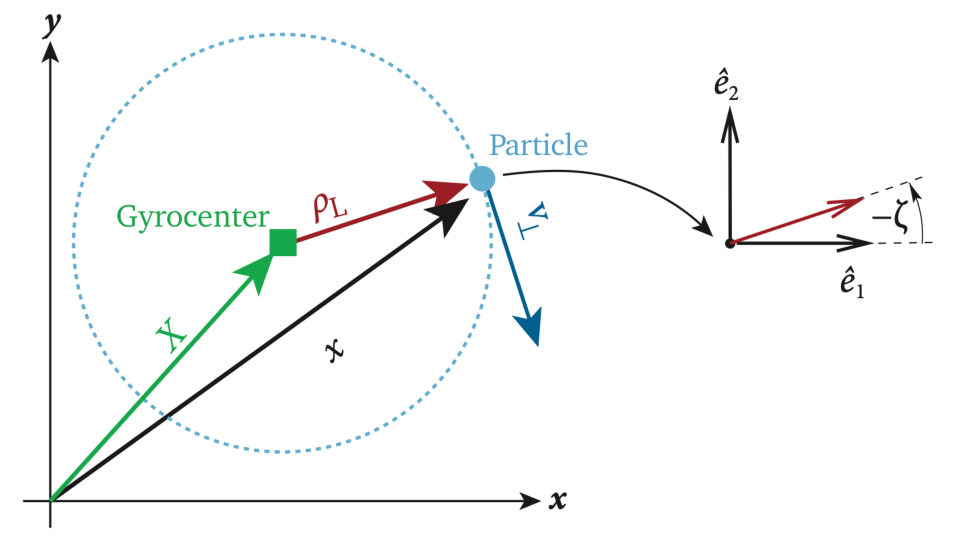
\includegraphics[width=0.85\paperwidth]{Theory/Gyro-Center-Coordinates.pdf}		
			\end{center}
		}

		\begin{tabular}{l l l}

			\onslide<2->{$\frac{\partial f}{\partial t} + \frac{\partial f}{\partial \vect{x}} \cdot \frac{\mathrm{d}\vect{x}}{\mathrm{d}t} + \frac{\partial f}{\partial \vect{v}} \cdot \frac{\mathrm{d}\vect{v}}{\mathrm{d}t} = 0$} & 
			\onslide<2->{$f(\vect{x}, \vect{v}, t)$} & 
			\onslide<2->{Vlasov Equation} \\[0.7cm]

			\multicolumn{2}{>{\onslide<3->}l<{\onslide}}{$\Downarrow$ \qquad $\frac{\omega}{\omega_\mathrm{c}} \sim \frac{k_\parallel}{k_\perp} \sim \frac{\rhoth}{L_\mathrm{n}} \sim \frac{\delta n}{n_0} \sim \frac{\delta B}{B_0} \sim \frac{v_\mathrm{d}}{\vth} \sim \epsilon_\mathrm{g}$} & 
			\onslide<3->{Gyrokinetic Ordering} \\[0.7cm]
			
			\onslide<5->{$\frac{\partial f}{\partial t} + \frac{\partial f}{\partial \vect{X}} \cdot \frac{\mathrm{d}\vect{X}}{\mathrm{d}t} + \frac{\partial f}{\partial v_\parallel} \cdot \frac{\mathrm{d}v_\parallel}{\mathrm{d}t} = 0$} & 
			\onslide<5->{$f(\vect{X}, v_{\parallel}, \mu)~;~\frac{\mathrm{d}\mu}{\mathrm{d}t} = 0$} & 
			\onslide<5->{Gyrokinetic Formalism} \\[0.7cm]
			
			\multicolumn{2}{>{\onslide<6->}l<{\onslide}}{$\Downarrow$ \qquad $f = f_0 + \delta f$} & 
			\onslide<6->{$\delta f$ Approx \& Local Limit} \\[0.7cm]

			\multicolumn{2}{>{\onslide<7->}l<{\onslide}}{$\frac{\partial g}{\partial t} + \vect{v}_\chi \cdot \nabla g + (v_\parallel \vect{b} + \vect{v}_\mathrm{D}) \cdot \nabla(\delta f) - \frac{\mu B}{m}\frac{\vect{B}\cdot\nabla B}{B^2}\frac{\partial (\delta f)}{\partial v_\parallel} = S$} &
			\onslide<7->{Gyrokinetic Equation} \\[0.7cm]
			\multicolumn{3}{>{\onslide<7->}l<{\onslide}}{$g \sim (f_0 + \delta f)\qquad S \sim (f + f_0)\qquad \vect{v}_\mathrm{D} \sim \nabla B \qquad \vect{v}_\chi \sim \exb \qquad f(\xcoord, \ycoord, s, v_\parallel, \mu)$} \\
		\end{tabular}
	\end{frame}

	\section*{Material and Methods}

	\begin{frame}
		\frametitle{Simulation Setup}

		\begin{center}
			\begin{itemize}
				\item <2-> Non-linear flux tube version of Gyrokinetic Workshop (GKW) 
				\item <3-> Circular concentric flux surfaces 
				\item <4-> Standard resolution with 6th order (S6) 
				\item <5-> Cyclone Base Case (CBC) parameters $\rlt = 6.0$ 
				\item <6-> Turbulence level is quantified by the turbulent heat conduction coefficient $\chi$ (normalized by $\rhoth^2 \vth/R$ ($\vth = \sqrt{2 T/m}$ and $\rhoth = \frac{m \vth}{|q|B}$)) 
				\item <7-> Quantities $\rhoth$, $R$, $T$, $\vth$ and $m$ are referenced quantities
				\item <8-> Standard box size $(L_\xcoord,~L_\ycoord) = (76.3,~89.8)\,\rhoth$
			\end{itemize}
			\onslide<4->{
			\bigskip
			\begin{tabular}{l | ccccc | ccccc | c | cc}
				& $N_\mathrm{m}$ & $N_x$ & $N_\mathrm{s}$ & $N_{\nu_\parallel}$ & $N_\mu$ & $D$ & $\nu_\mathrm{d}$           & $D_{\nu_\parallel}$ & $D_x$ & $D_y$ & Order & $k_y\rho$ & $k_x\rho$ \\
				\hline
				S6   & 21    & 83    & 16    & 64                  & 9       & 1   & $|\nu_\parallel|$ & 0.2                 & 0.1   & 0.1   & 6     & 1.4       & 2.1       \\
			\end{tabular}}
		\end{center}
	\end{frame}

	\begin{frame}
		\frametitle{Diagnostics}
		
		\begin{center}
			\onslide<2-> $\wexb = \sum_{\kzf} \hatwexb(\kzf,t) \, \exp(\mathrm{i} \kzf \xcoord)$ \\[0.5cm]
			\onslide<2-> $\kzf = 2\pi \nzf/L_\xcoord$ \\[0.5cm]
			\onslide<2-> $\hatwexbamp = 2 |\hatwexb(\kzf,t)|$ \\[0.5cm]
			\begin{itemize}
				\item <3-> Zonal flow mode that dominates the $\exb$ staircase pattern are called \textbf{basic mode} 
				\item <4-> The basic mode exhibits the maximum amplitude in the spectrum $\hatwexbamp$
			\end{itemize}
		\end{center}
	\end{frame}
	\begin{frame}
		\frametitle{Restart Script}
		\pause
		
		\newcommand{\distance}{2.5cm}

		\begin{center}
		    \begin{tikzpicture}[node distance=1.5cm]
			
		        \node (init)         [init]                                                 {Start / Initialize};
		        \node (startLoop)    [startstop, below of = init]                           {Loop};
		        \node (checkStatus)  [process, below of=startLoop]                          {Check Status};
		        \node (checkData)    [process, below of=checkStatus, yshift = -1.5cm]       {Check Data};
		        \node (checkPending) [decision, below of=checkStatus, xshift=\distance]     {Pending};
		        \node (checkRunning) [decision, below of=checkStatus, xshift=-\distance]    {Running};
			
			
		        \draw [arrow] (init)           --                                           (startLoop);
		        \draw [arrow] (startLoop)      --                                           (checkStatus);
		        \draw [arrow] (checkStatus)    -|                                           (checkRunning);
		        \draw [arrow] (checkRunning)   -- node[anchor=south] {No}                   (checkPending);
		        \draw [arrow] (checkPending)   -- node[anchor=north west] {Yes} + ( 3,0) |- (startLoop);
		        \draw [arrow] (checkRunning)   -- node[anchor=north east] {Yes} + (-3,0) |- (startLoop);
		        \draw [arrow] (checkPending)   |- node[anchor=north west] {No}              (checkData);
			
		    \end{tikzpicture}
		\end{center}
	\end{frame}

	\begin{frame}
		\frametitle{Restart Script}

		\newcommand{\distance}{2.5cm}

		\begin{center}
		    \begin{tikzpicture}[node distance=2cm]
			
		        \node (checkData)    [process]       										{Check Data};
		        \node (error)        [decision, below of=checkData, xshift=-\distance]      {Errors};
		        \node (checkPoint)   [decision, below of=checkData, xshift=\distance]       {Checkpoint};
		        \node (backup)       [process,  below of=error, xshift=-\distance]          {Backup Data};
		        \node (restore)      [process,  below of=checkPoint, xshift=\distance]      {Restore Data};
		        \node (reset)        [process,  below of=checkData, yshift=-2cm]            {Reset Data};
		        \node (checkStep)    [decision, below of = reset]                           {Enough Timesteps};

		        \draw [arrow] (checkData)      -|                                           (error);
		        \draw [arrow] (error)          -- node[anchor=south] {Yes}                  (checkPoint);
		        \draw [arrow] (error)          -| node[anchor=south east] {No}              (backup);
		        \draw [arrow] (checkPoint)     -| node[anchor=south west] {No}              (restore);
		        \draw [arrow] (checkPoint)     |- node[anchor=north west] {Yes}             (reset);
		        \draw [arrow] (backup)         --                                           (checkStep);
		        \draw [arrow] (reset)          --                                           (checkStep);
		        \draw [arrow] (restore)        --                                           (checkStep);
			
		    \end{tikzpicture}
		\end{center}

	\end{frame}

	\begin{frame}
		\frametitle{Restart Script}

		\newcommand{\distance}{2.5cm}

		\begin{center}
		    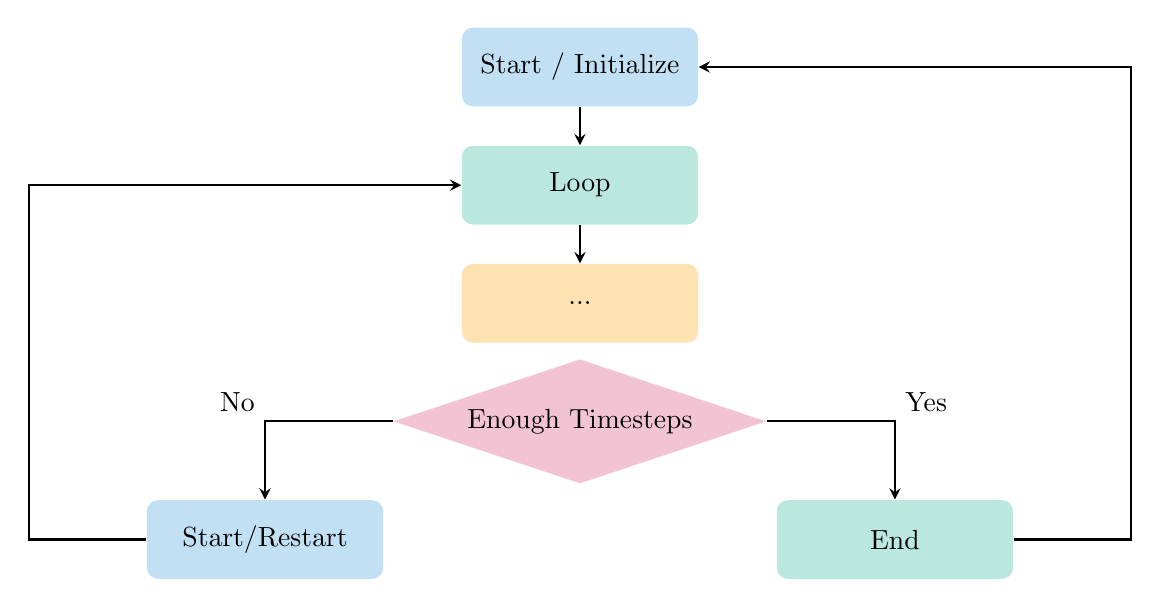
\begin{tikzpicture}[node distance=1.5cm]
				
				\node (init)         [init]                                                 {Start / Initialize};
		        \node (startLoop)    [startstop, below of = init]                           {Loop};
		        \node (checkStatus)  [process, below of=startLoop]                          {...};
		        \node (checkStep)    [decision, below of = checkStatus]                     {Enough Timesteps};
		        \node (end)          [startstop, below of=checkStep, xshift=4cm]            {End};
		        \node (restart)      [init, below of=checkStep, xshift=-4cm]                {Start/Restart};

		        \draw [arrow] (init)           --                                           (startLoop);
		        \draw [arrow] (startLoop)      --                                           (checkStatus);
		        \draw [arrow] (checkStep)      -| node[anchor=south east] {No}              (restart);
		        \draw [arrow] (checkStep)      -| node[anchor=south west] {Yes}             (end);
		        \draw [arrow] (restart)        -- + (-3,0) |-                               (startLoop);
		        \draw [arrow] (end)            -- + ( 3,0) |-                               (init);
			
		    \end{tikzpicture}
		\end{center}

	\end{frame}

	\section*{Results}

	\begin{frame}
		\frametitle{Variation of Computational Resolution}
		\pause
		\textbf{Goals:}
		\begin{itemize}
			\item Estimate the minimal resolution without numerical dissipation
			\item Reduce \textbf{calculation time} and \textbf{costs} of the simulation
		\end{itemize}
		\pause
		\textbf{Criteria:}
		\begin{enumerate}
			\item[\textbf{(1)}] Subdued turbulence after \textbf{short} time periods
			\item[\textbf{(2)}] Stability for \textbf{long} time periods 
		\end{enumerate}
		\pause
		\textbf{Verification:}
		\begin{enumerate}
			\item Reduce only one number of grid points and look if criterias \textbf{(1), (2)} are satisfied
			\item Reduce to known the minimum number of grid points to verify result in general.
		\end{enumerate}
	\end{frame}

	\begin{frame}
		\frametitle{Benchmark}
		\begin{center}
			\only<2>{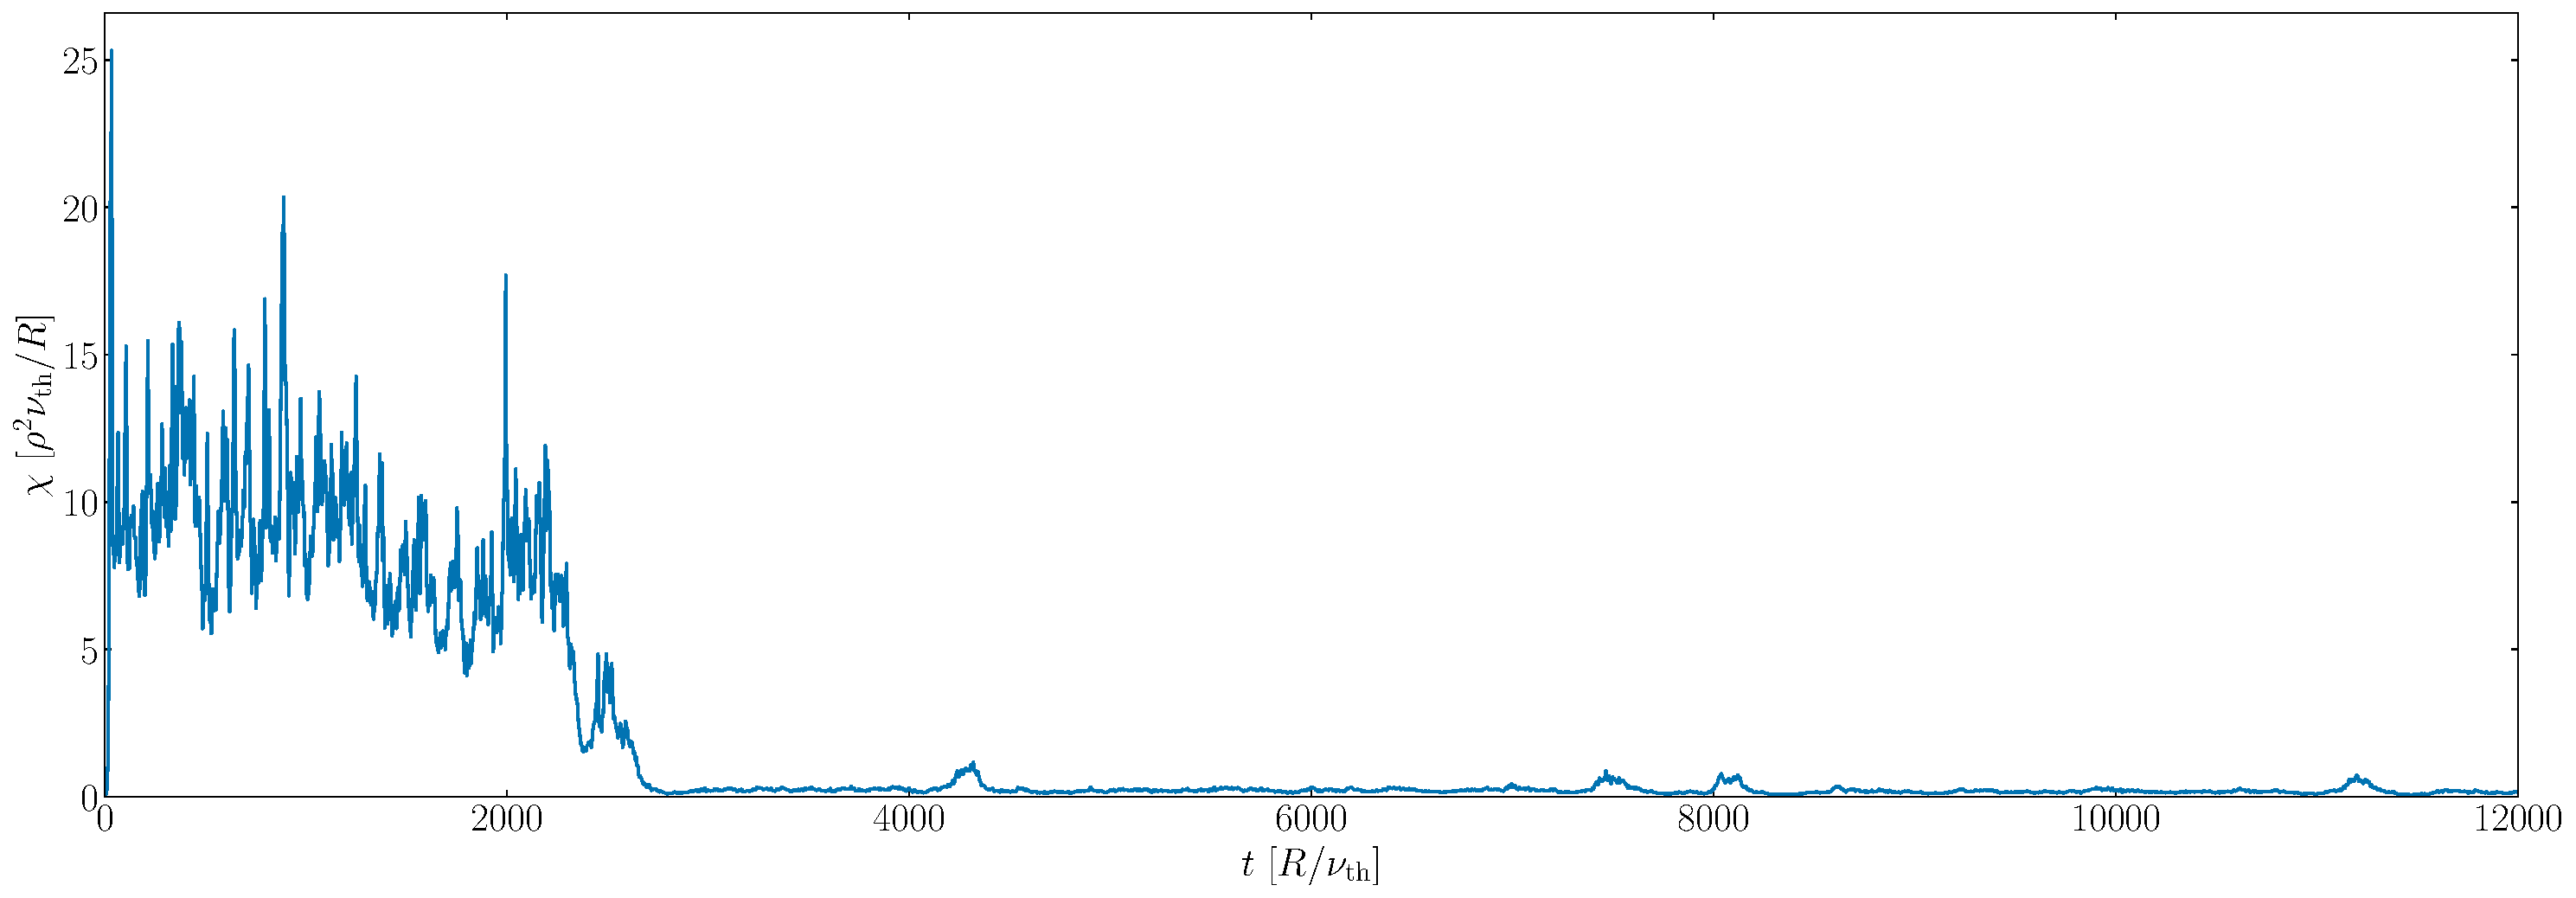
\includegraphics[width = 0.8\paperwidth]{S6_rlt6.0/boxsize1x1/Ns16/Nvpar64/Nmu9/S6_rlt6.0_boxsize1x1_Ns16_Nvpar64_Nmu9_eflux.pdf}}

			\only<3>{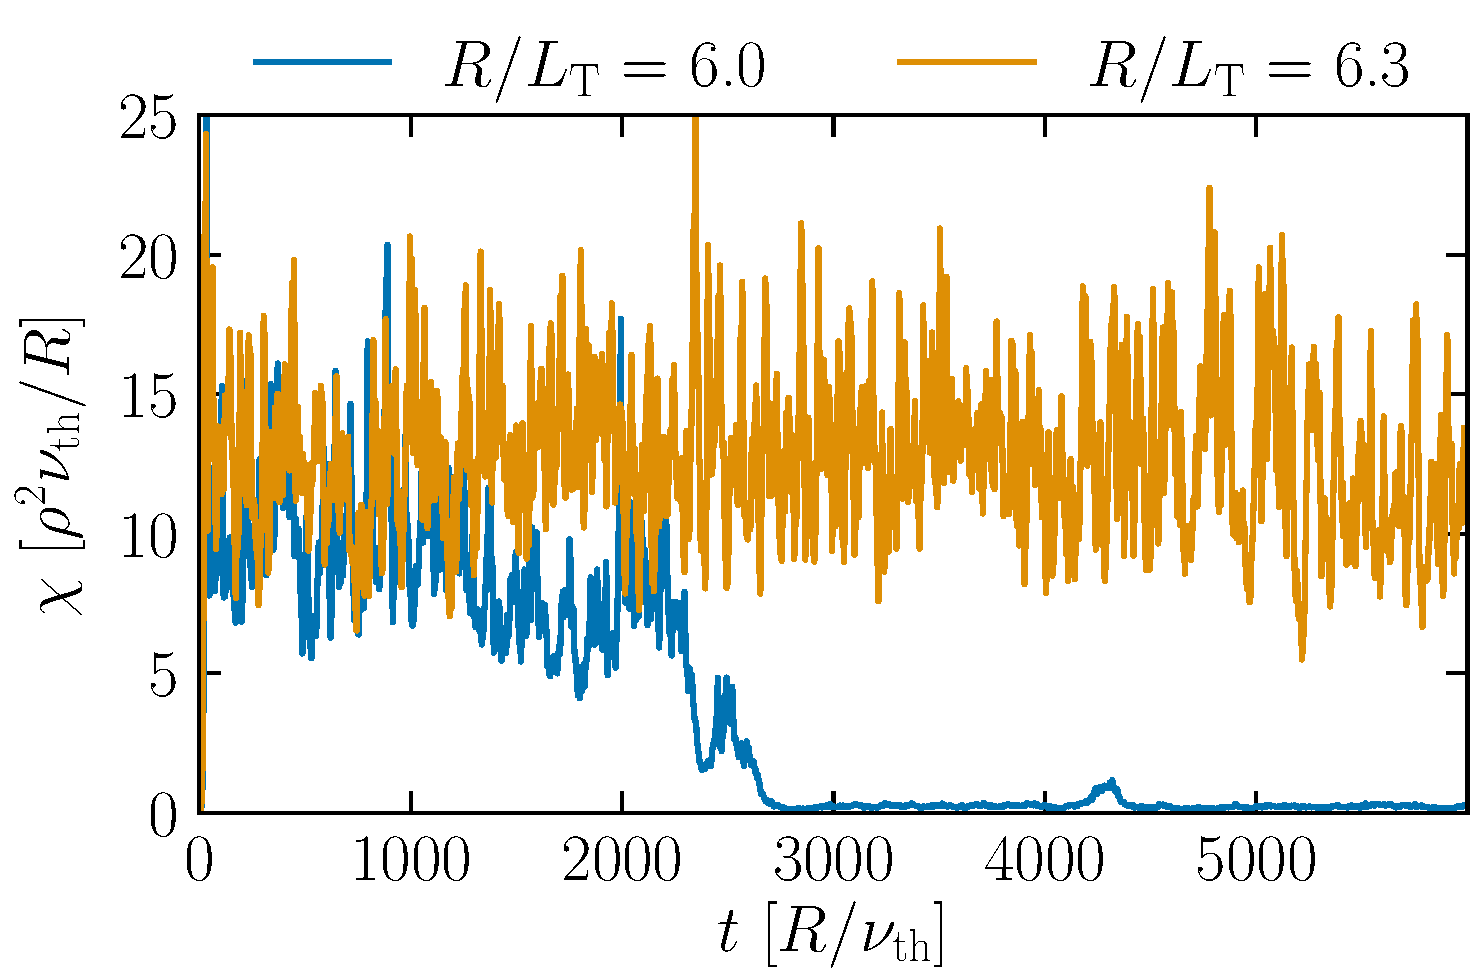
\includegraphics[width = 0.8\paperwidth]{Comparison/Gradient-Length/S6_rlt6.0-6.3_boxsize1x1_Ns16_Nvpar64_Nmu9_eflux_comparison.pdf}}
		\end{center}
	\end{frame}

	\begin{frame}
		\frametitle{Reduction of Grid Points}
		
		\begin{center}
			\only<2>{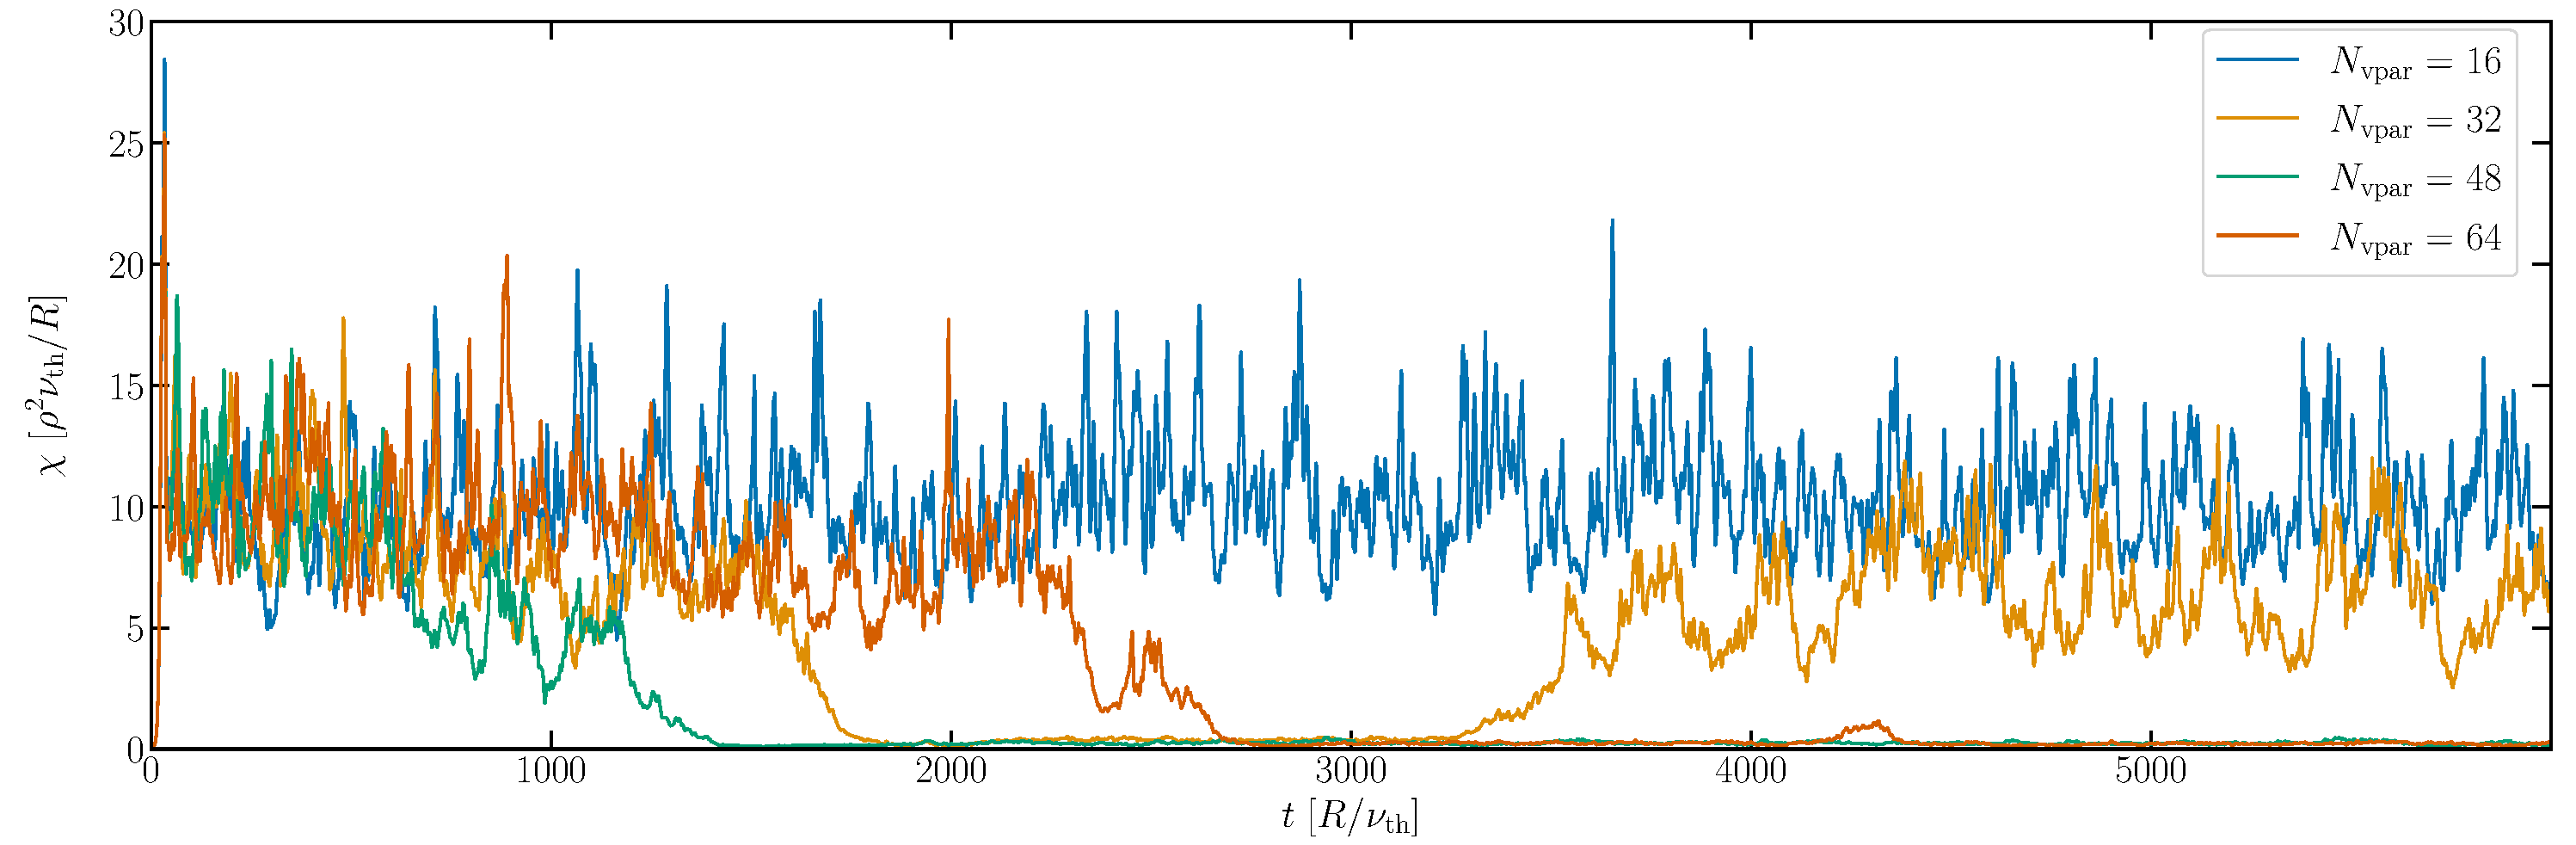
\includegraphics[width = 0.8\paperwidth]{Comparison/Resolution/Nvpar/S6_rlt6.0_boxsize1x1_Ns16_Nvpar16-32-48-64_Nmu9_eflux_comparison.pdf}}

			\only<3>{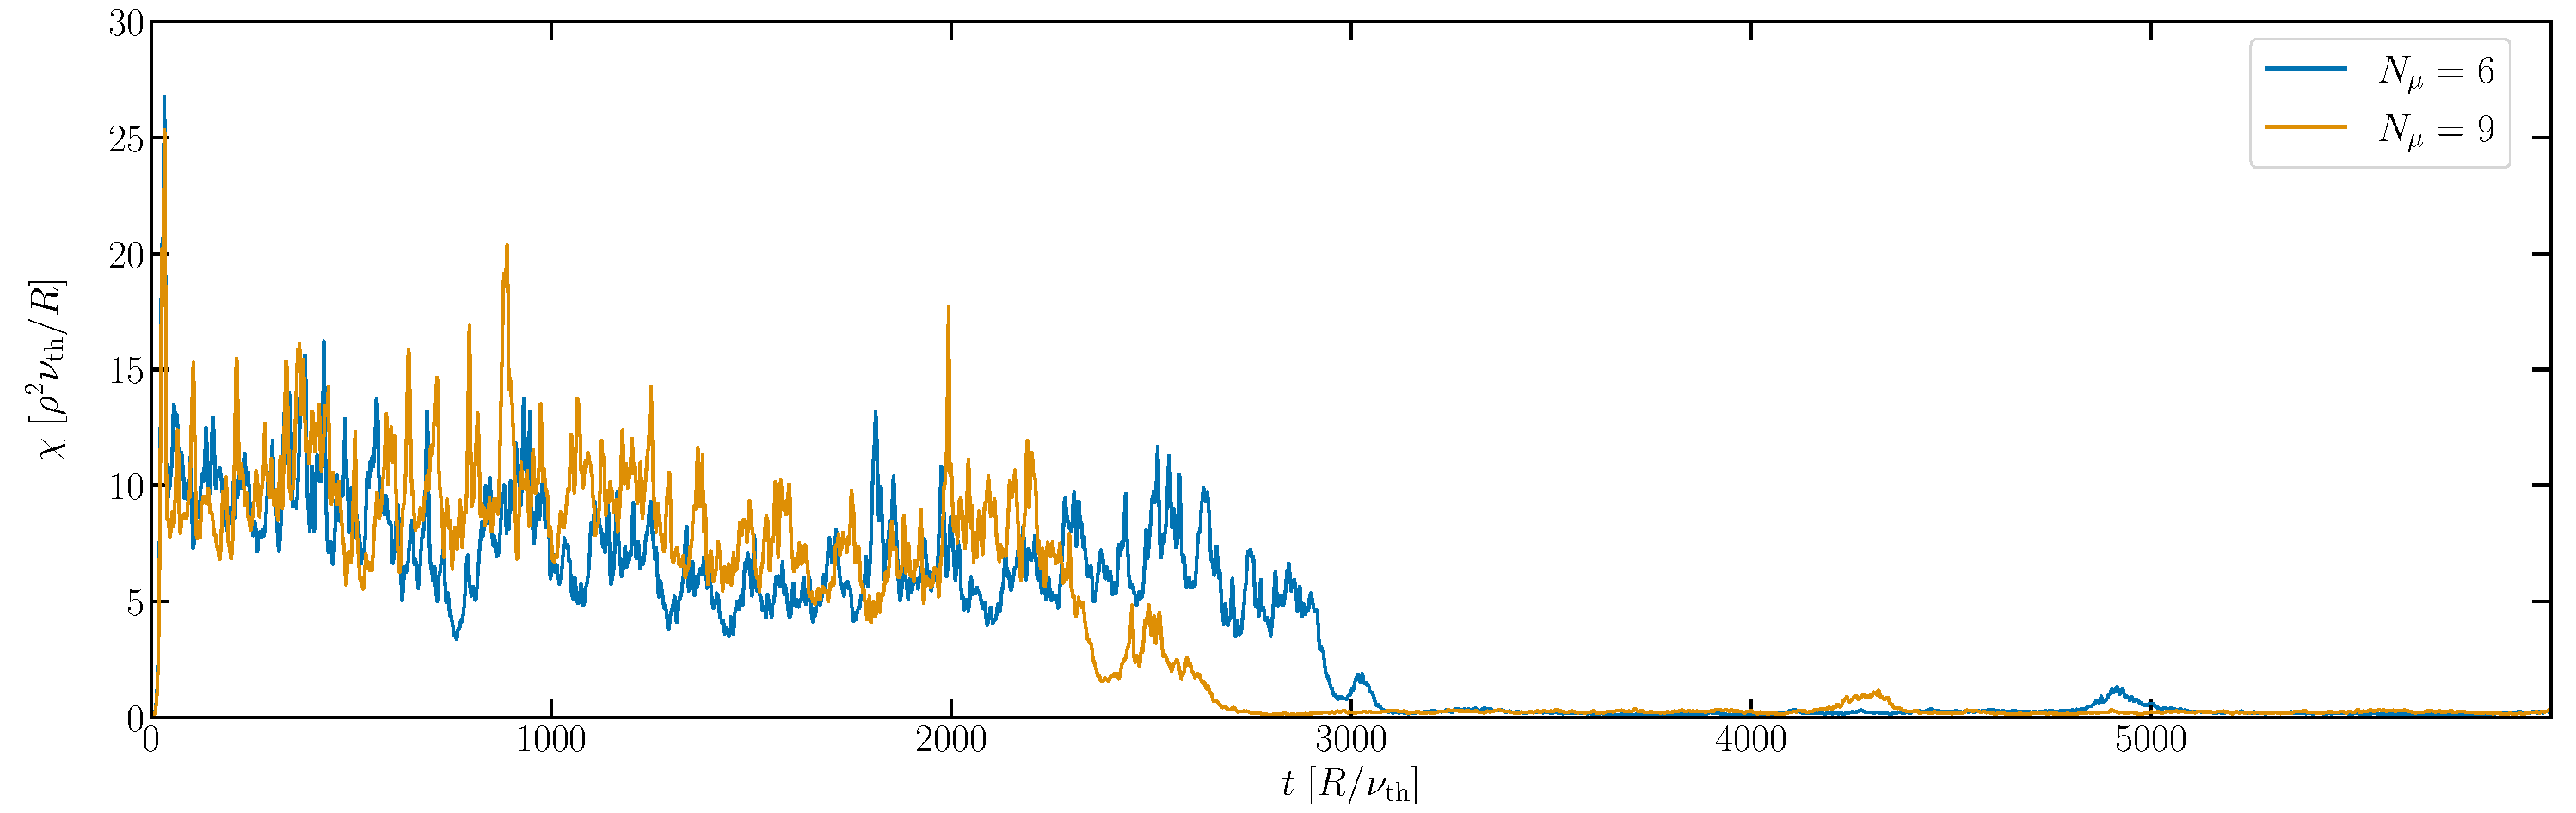
\includegraphics[width = 0.8\paperwidth]{Comparison/Resolution/Nmu/S6_rlt6.0_boxsize1x1_Ns16_Nvpar64_Nmu6-9_eflux_comparison.pdf}}
			
			\only<4>{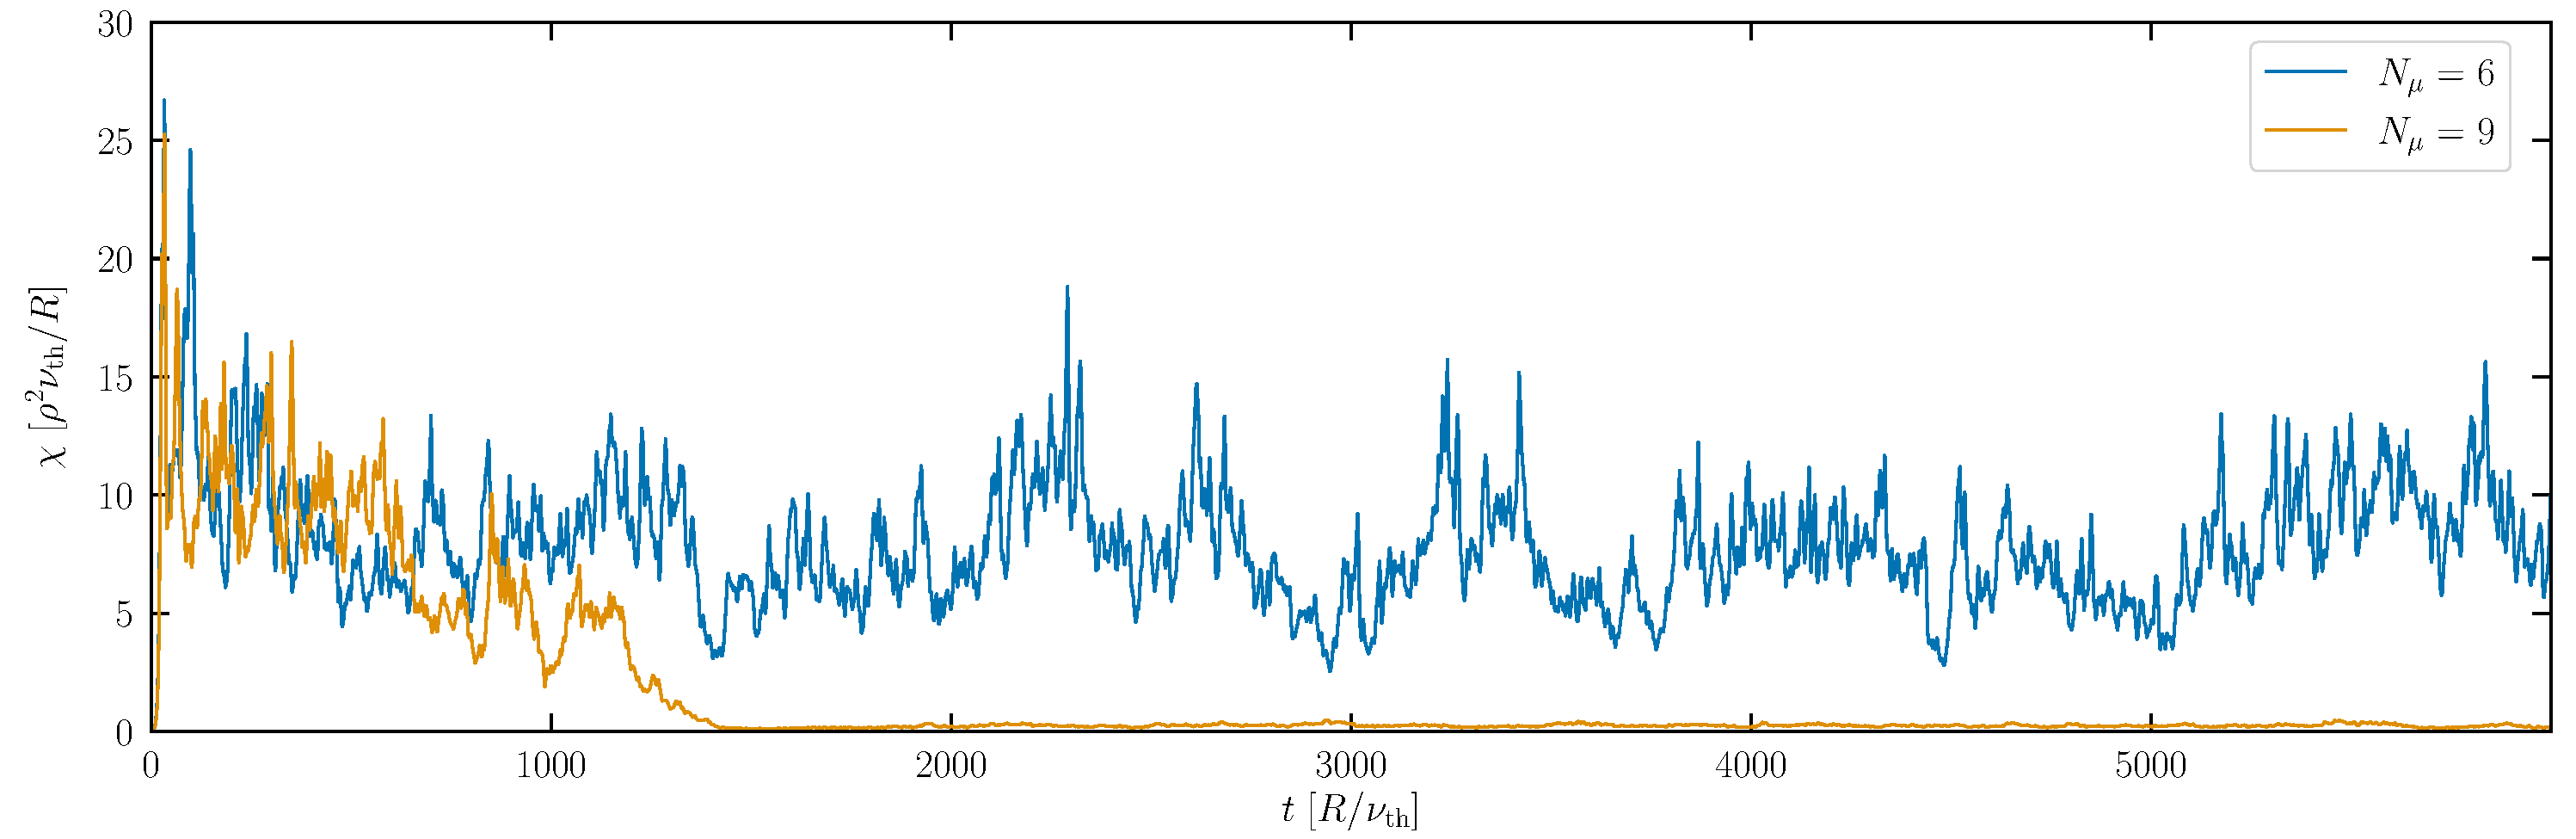
\includegraphics[width = 0.8\paperwidth]{Comparison/Resolution/Nmu/S6_rlt6.0_boxsize1x1_Ns16_Nvpar48_Nmu6-9_eflux_comparison.pdf}}
			
			\only<5>{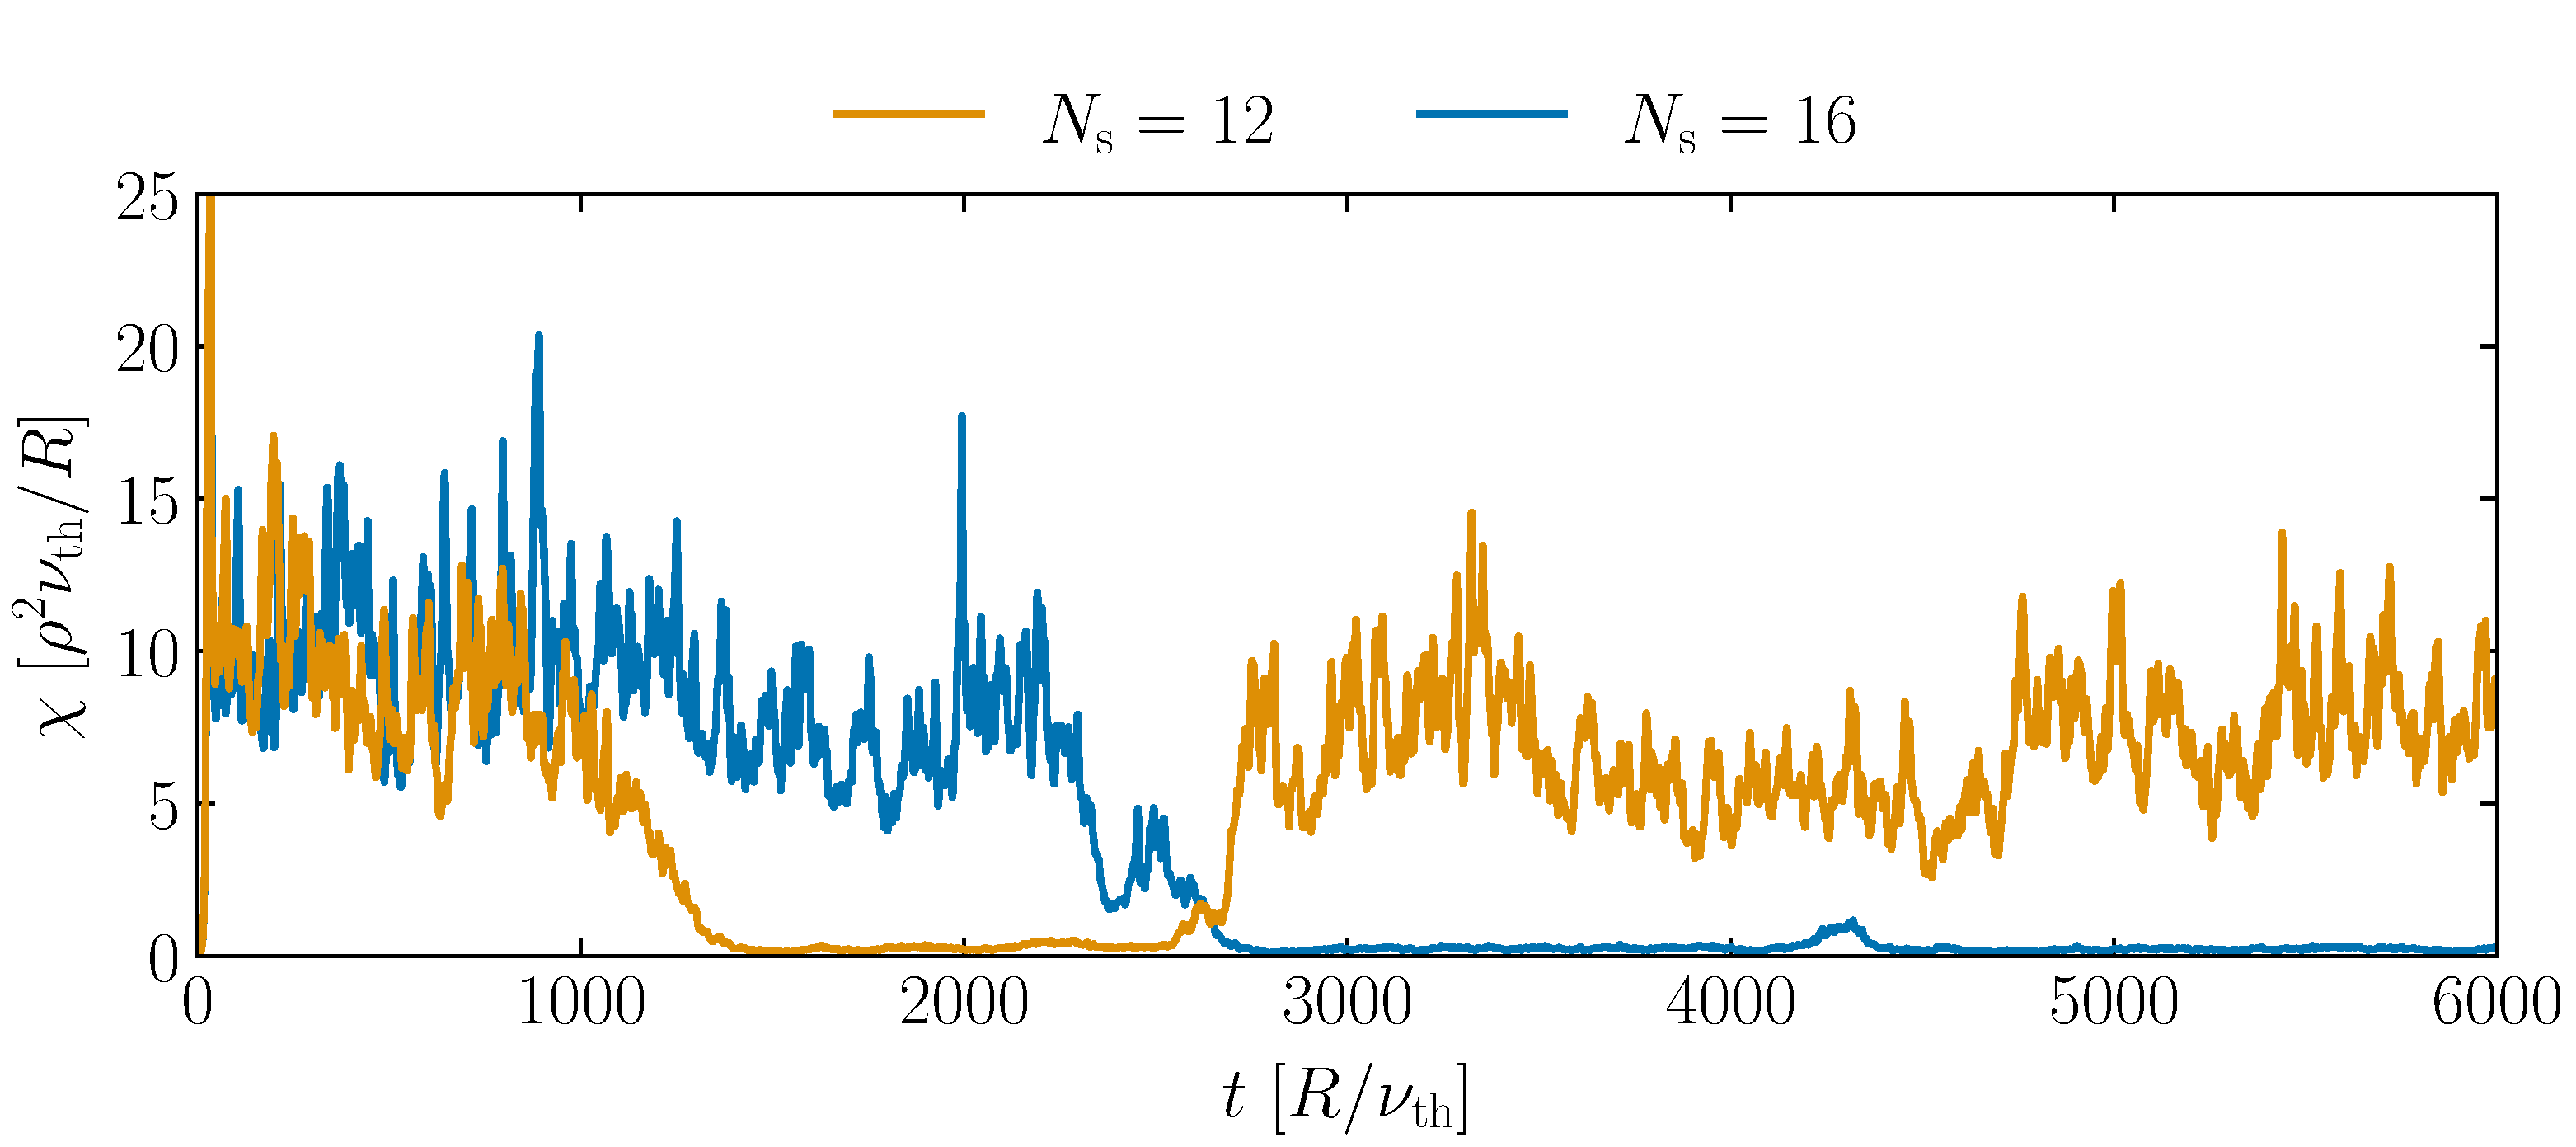
\includegraphics[width = 0.8\paperwidth]{Comparison/Resolution/Ns/S6_rlt6.0_boxsize1x1_Ns12-16_Nvpar64_Nmu9_eflux_comparison.pdf}}
			
			\only<6>{
				\textbf{Final Resolution}\\
				\bigskip
				\begin{tabular}{l | ccccc | ccccc | c | cc}
					& $N_\mathrm{m}$ & $N_x$ & $N_\mathrm{s}$ & $N_{\nu_\parallel}$ & $N_\mu$ & $D$ & $\nu_\mathrm{d}$           & $D_{\nu_\parallel}$ & $D_x$ & $D_y$ & Order & $k_y\rho$ & $k_x\rho$ \\
					\hline
					S6   & 21    & 83    & 16    & 48                  & 9       & 1   & $|\nu_\parallel|$ & 0.2                 & 0.1   & 0.1   & 6     & 1.4       & 2.1       \\
				\end{tabular}
			}
		\end{center}
	\end{frame}

	\begin{frame}
		\frametitle{Size Convergence of $\exb$ Staircase Pattern}
		\begin{center}
			\only<2>{\textbf{(1) Radial} \\[0.5cm] $\NR \times \NB \in [1\times1,~2\times1,~3\times1,~4\times1]$}

			\only<3>{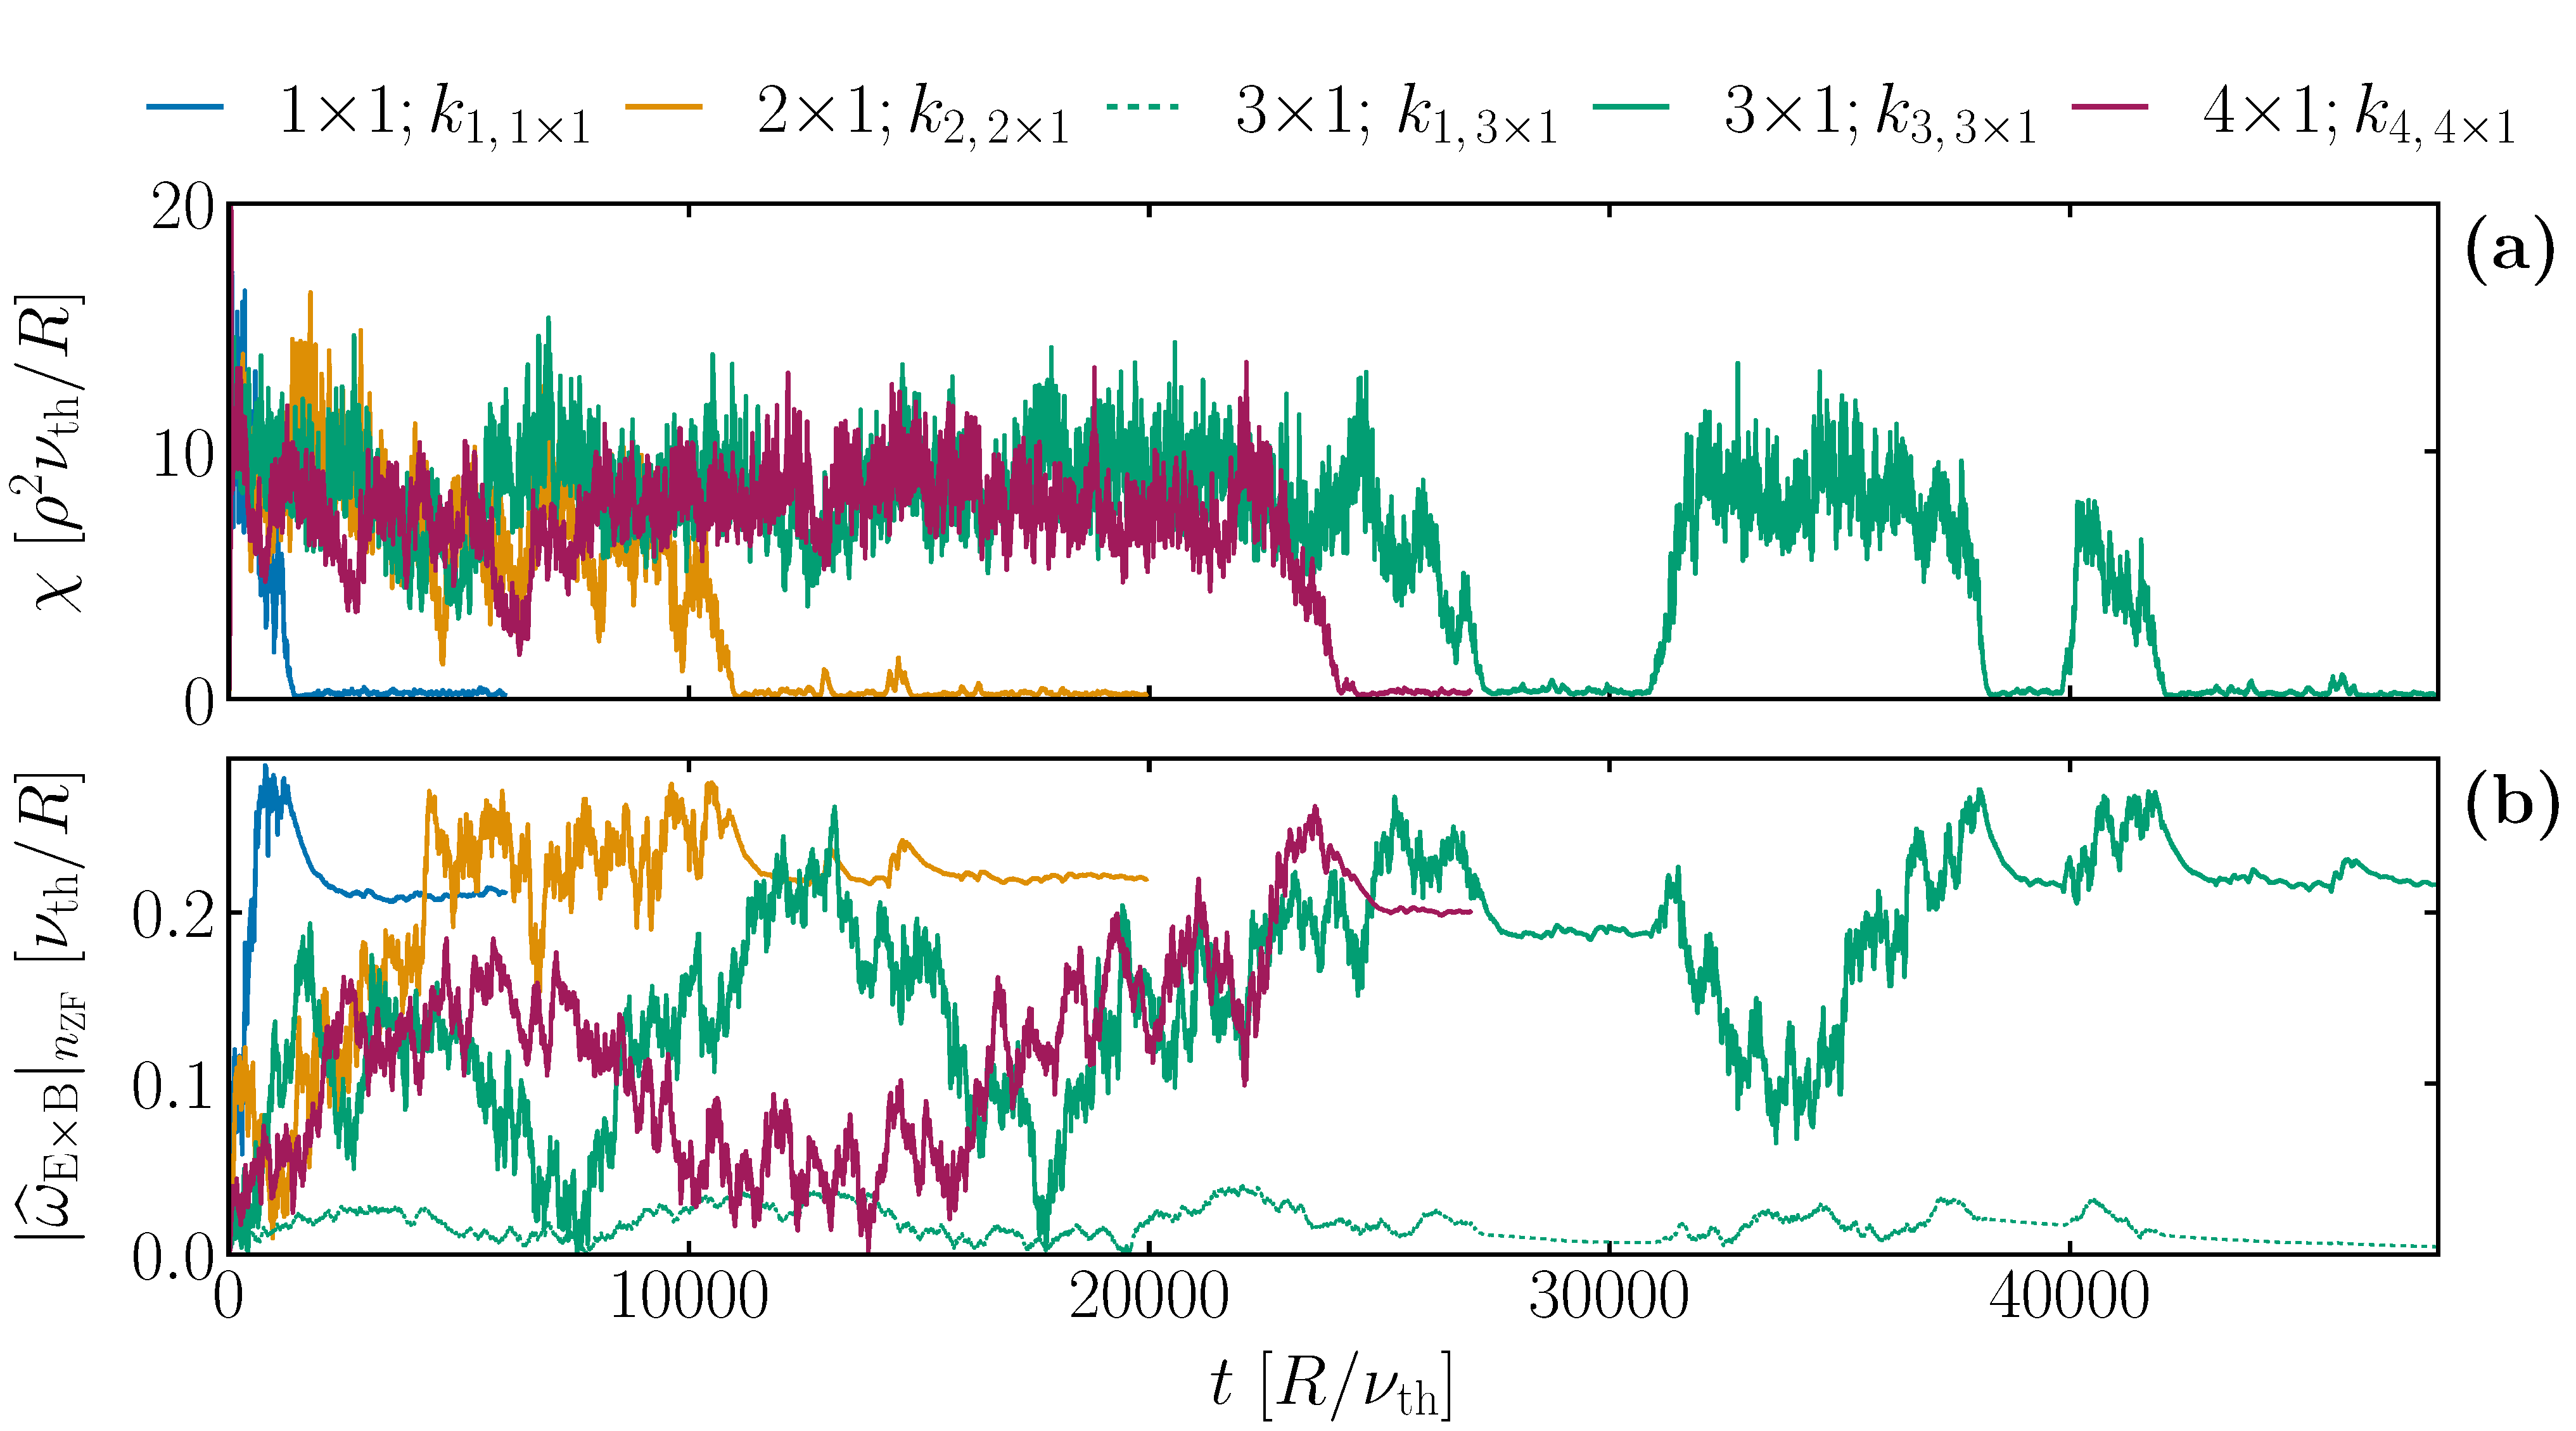
\includegraphics[width = 0.8\paperwidth]{Comparison/Boxsize/S6_rlt6.0_boxsize1-2-3-4x1_Ns16_Nvpar48_Nmu9_comparison_thesis.pdf}}

			\only<4>{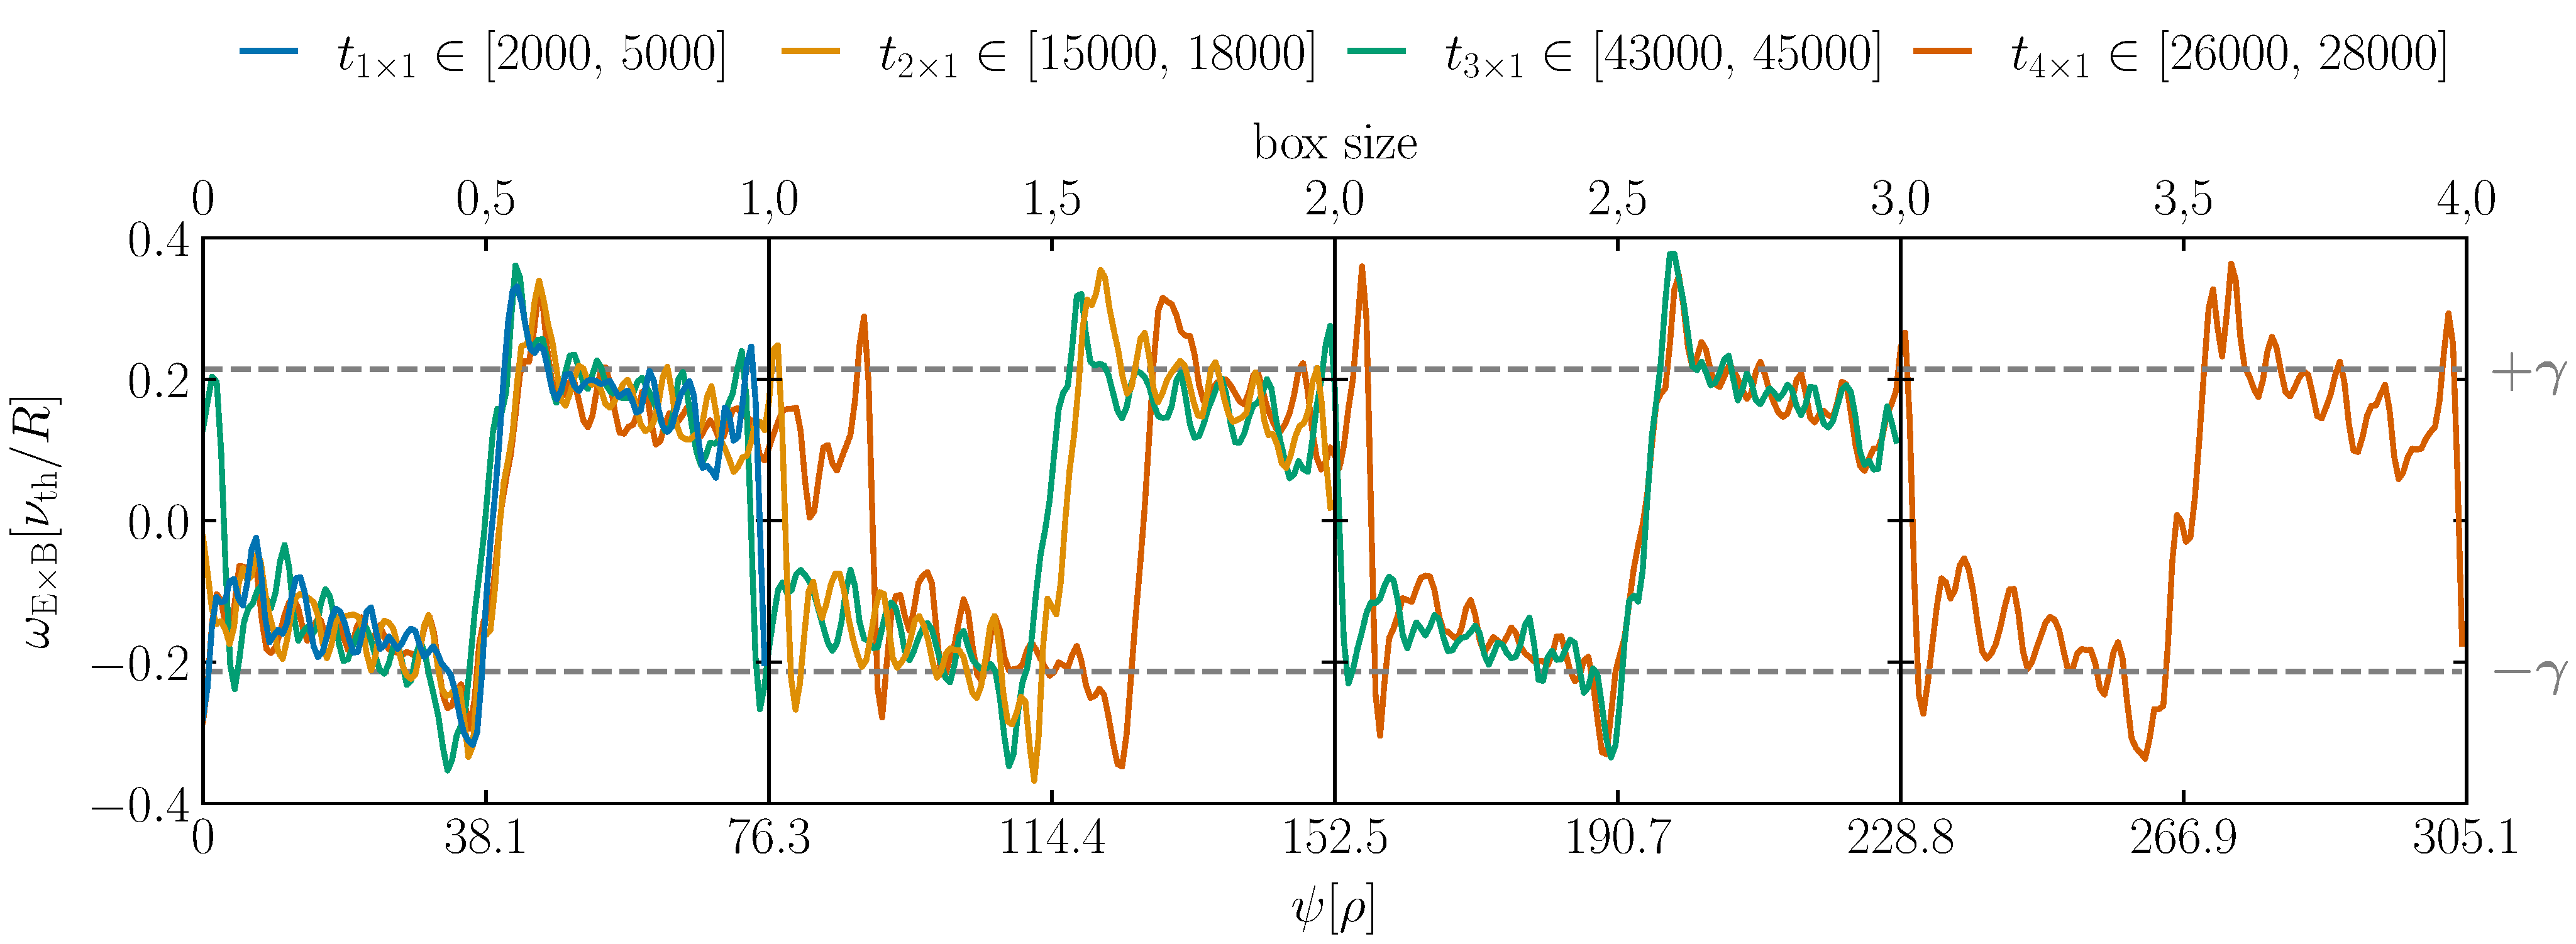
\includegraphics[height = 0.5\paperheight]{Comparison/Boxsize/S6_rlt6.0_boxsize1-2-3-4x1_Ns16_Nvpar48_Nmu9_wexb_comparison.pdf}}

			\only<5>{\textbf{(2) Isotropic} \\[0.5cm] $\NR \times \NB \in [1\times1,~1.5\times1.5,~2\times2,~2.5\times2.5,~3\times3]$}

			\only<6>{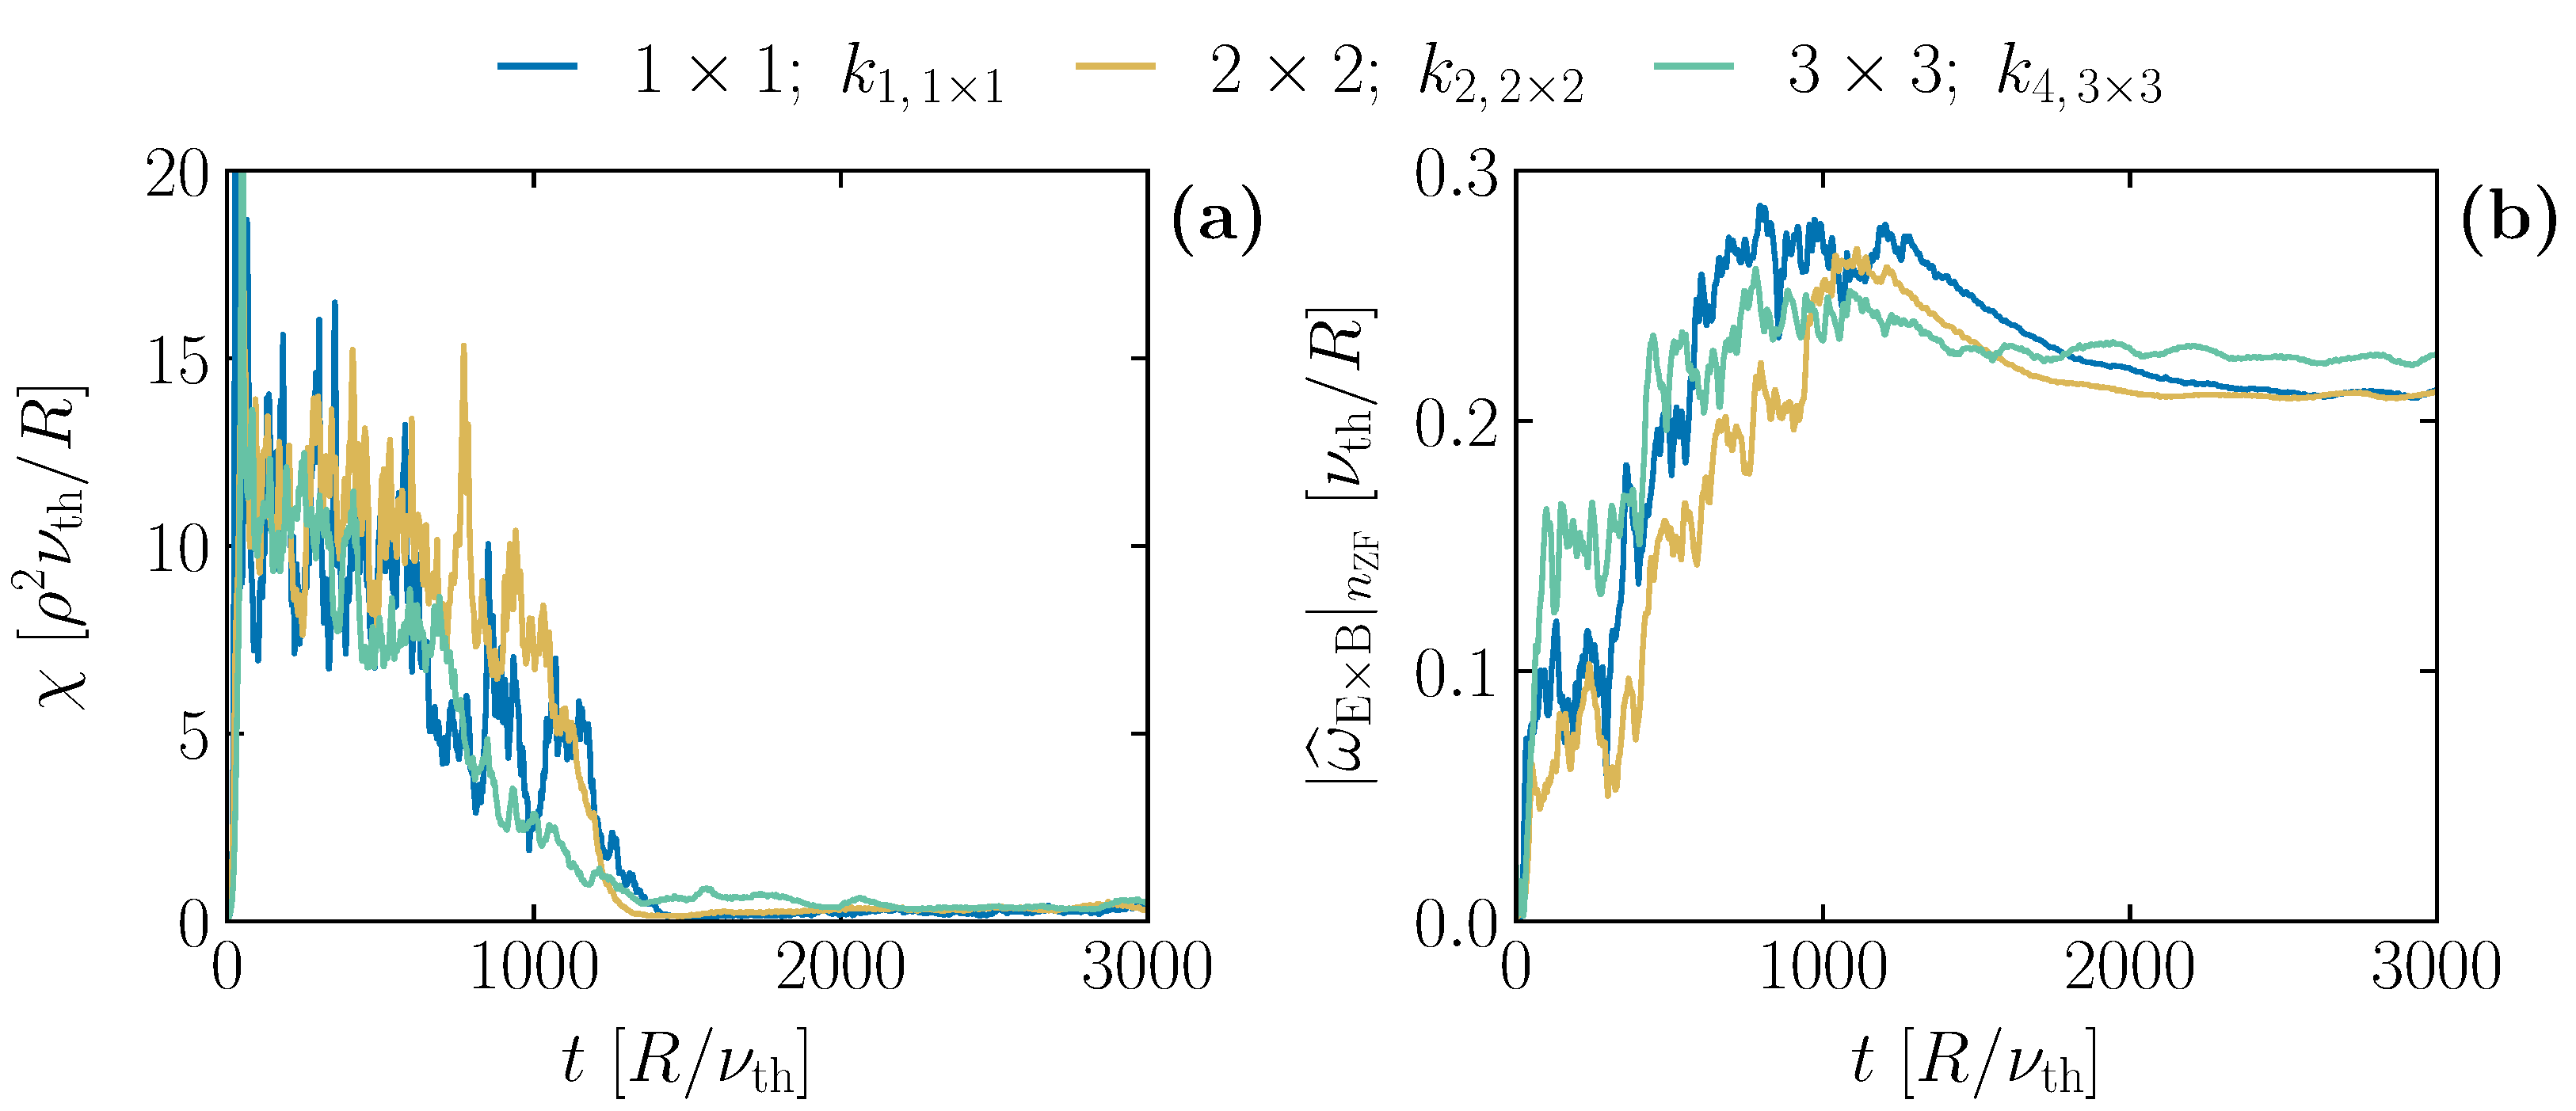
\includegraphics[width = 0.8\paperwidth]{Comparison/Boxsize/S6_rlt6.0_boxsize1x1-2x2-3x3_Ns16_Nvpar48_Nmu9_comparison_thesis.pdf}}

			\only<7>{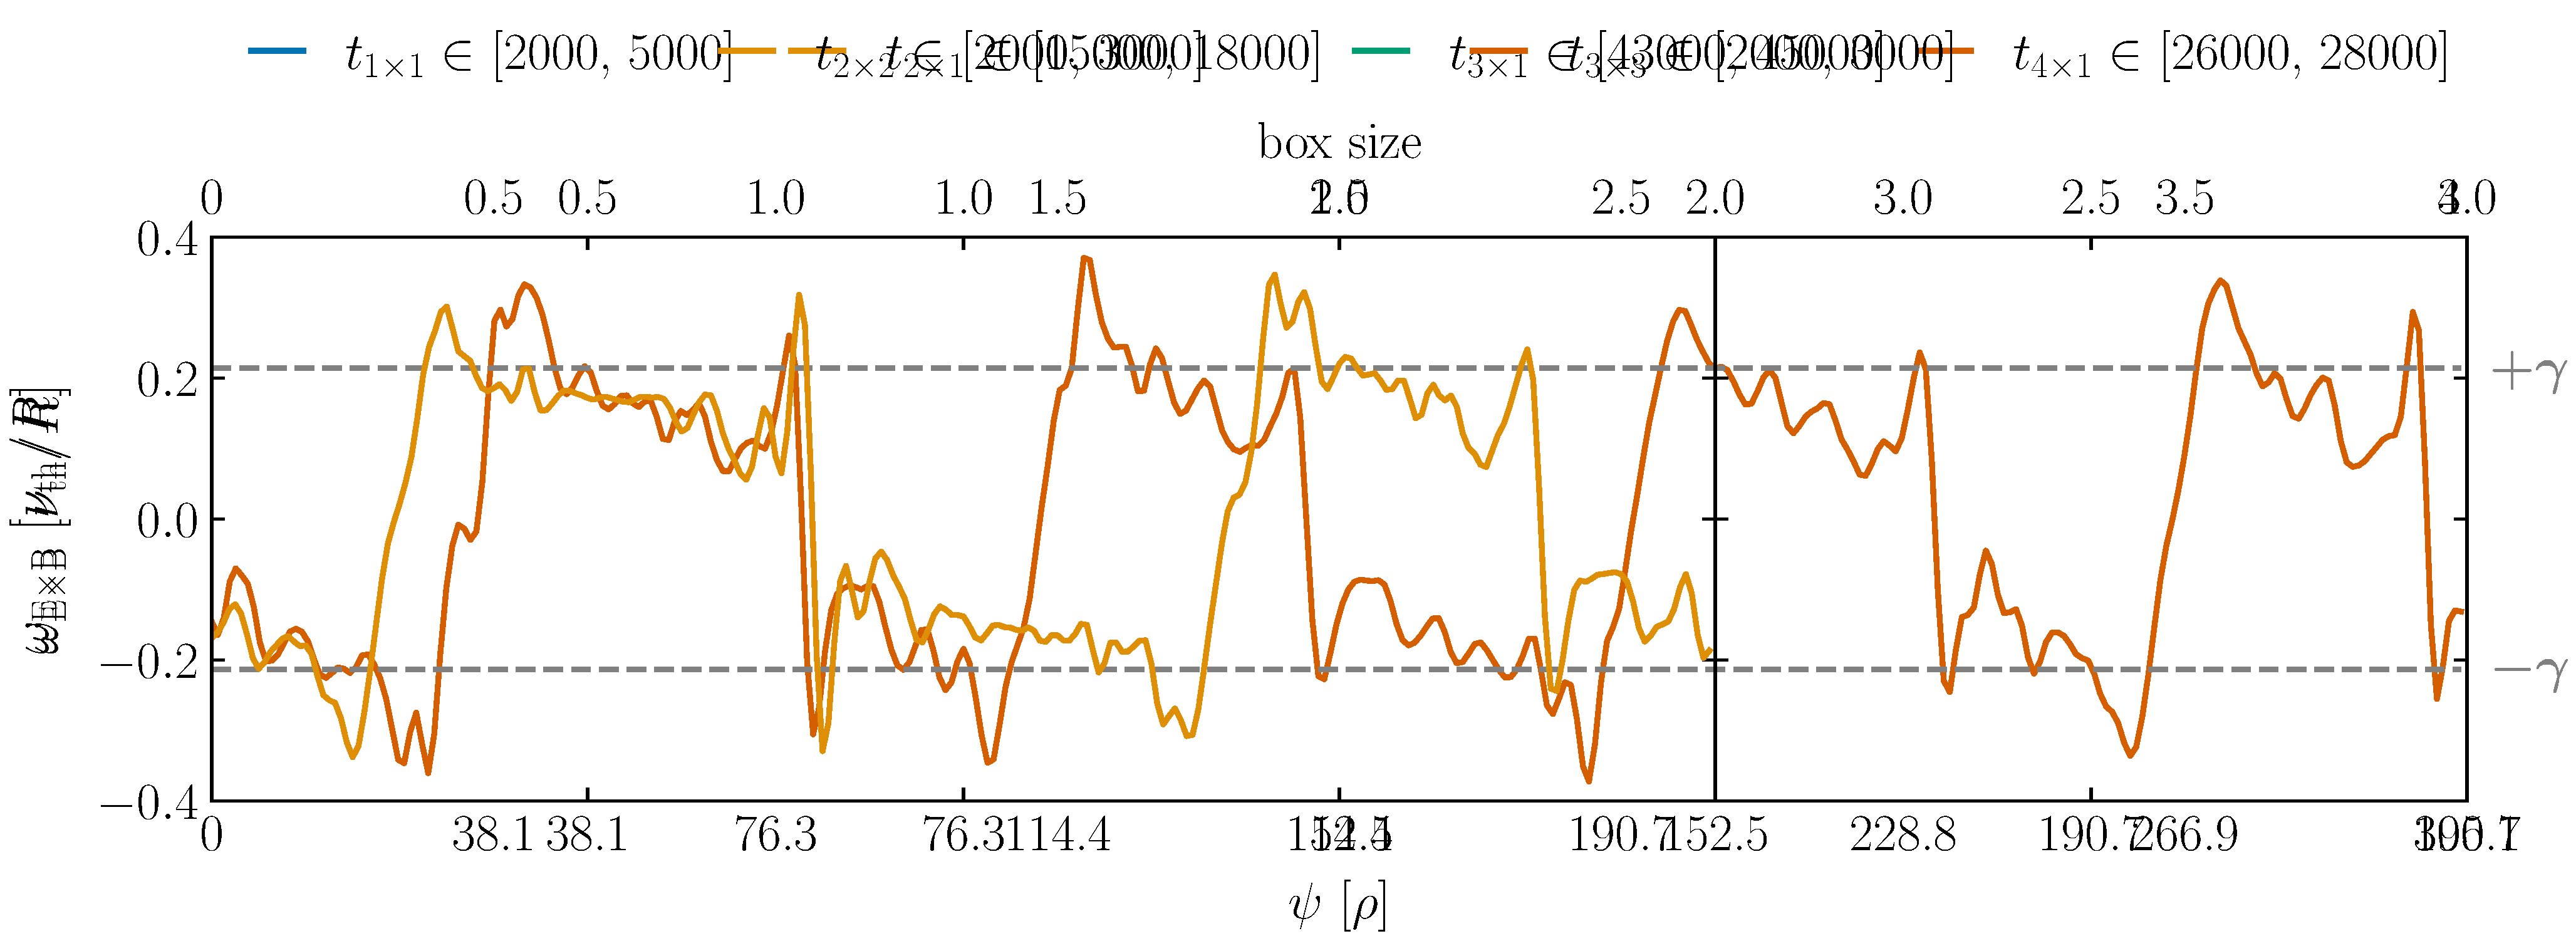
\includegraphics[height = 0.5\paperheight]{Comparison/Boxsize/S6_rlt6.0_boxsize1x1-2x2-3x3_Ns16_Nvpar48_Nmu9_wexb_comparison.pdf}}

			\only<8>{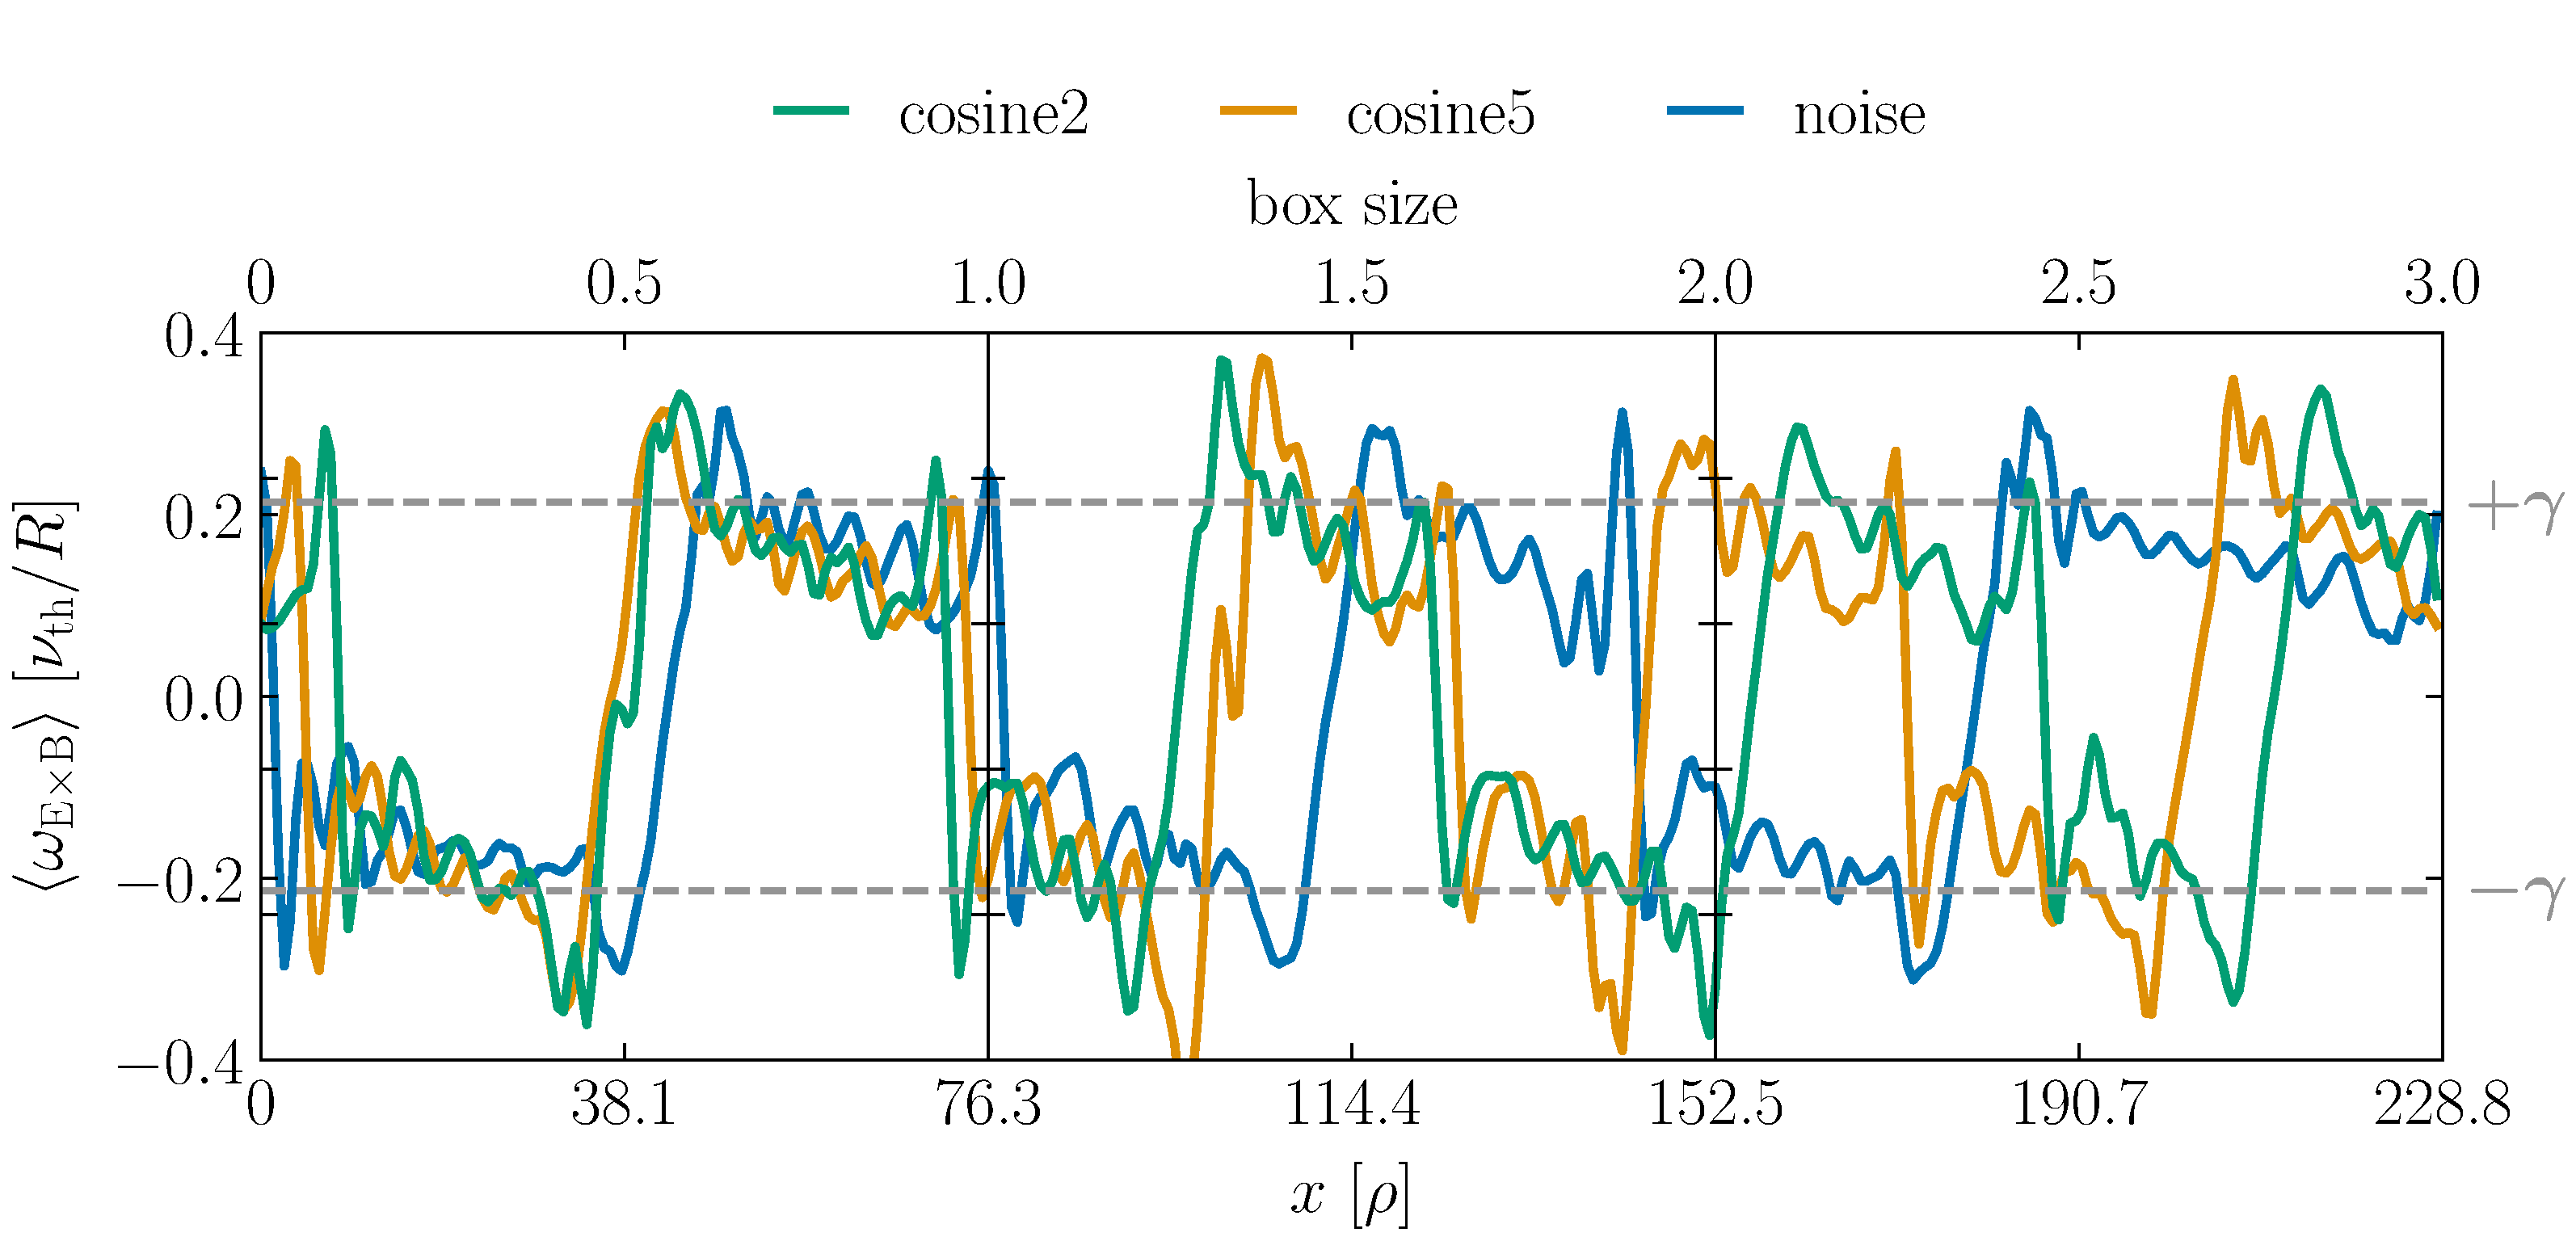
\includegraphics[height = 0.5\paperheight]{Comparison/Boxsize/S6_rlt6.0_boxsize3x3_Ns16_Nvpar48_Nmu9_cosine2-cosine5-noise_wexb_comparison.pdf}}

			\only<9>{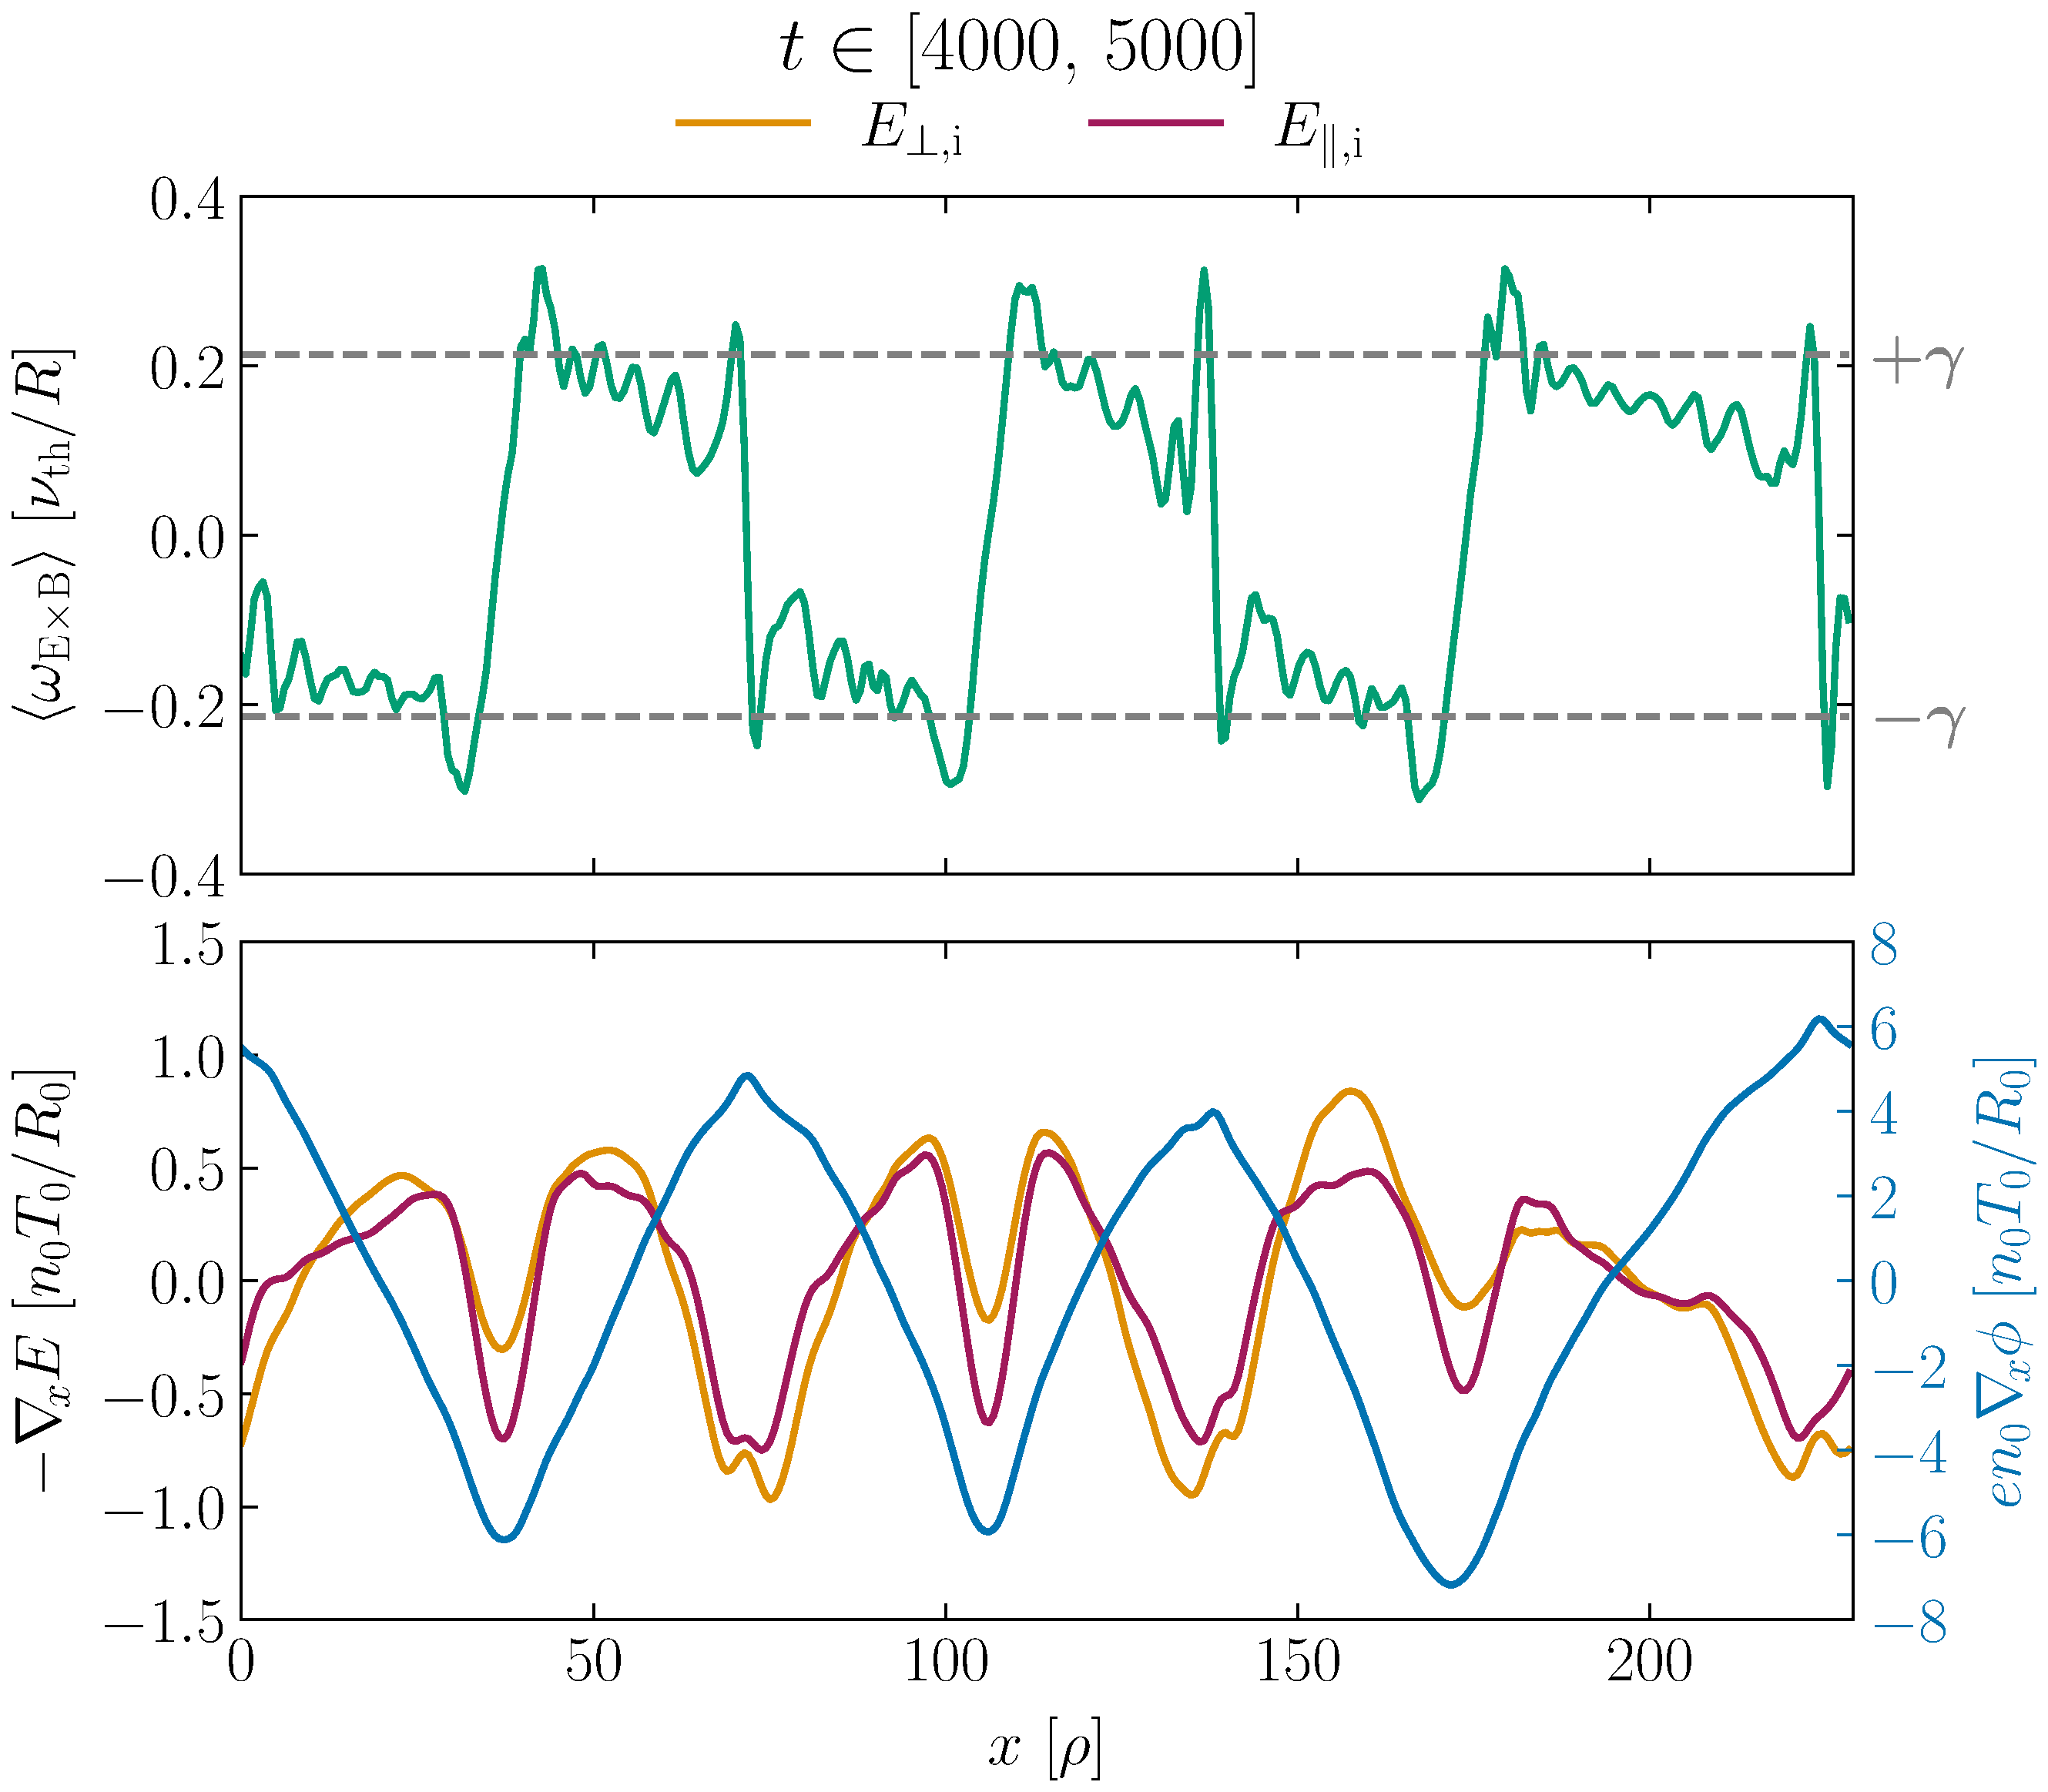
\includegraphics[height = 0.7\paperheight]{S6_rlt6.0/boxsize3x3/Ns16/Nvpar48/Nmu9/noise/S6_rlt6.0_boxsize3x3_Ns16_Nvpar48_Nmu9_noise_wexb_dens_ene_selection.pdf}}
			
			\only<10>{\textbf{(3) Binormal} \\[0.5cm] $\NR \times \NB \in [3\times1.5,~3\times2.5,~3\times3,~3\times5]$}
			
			\only<11>{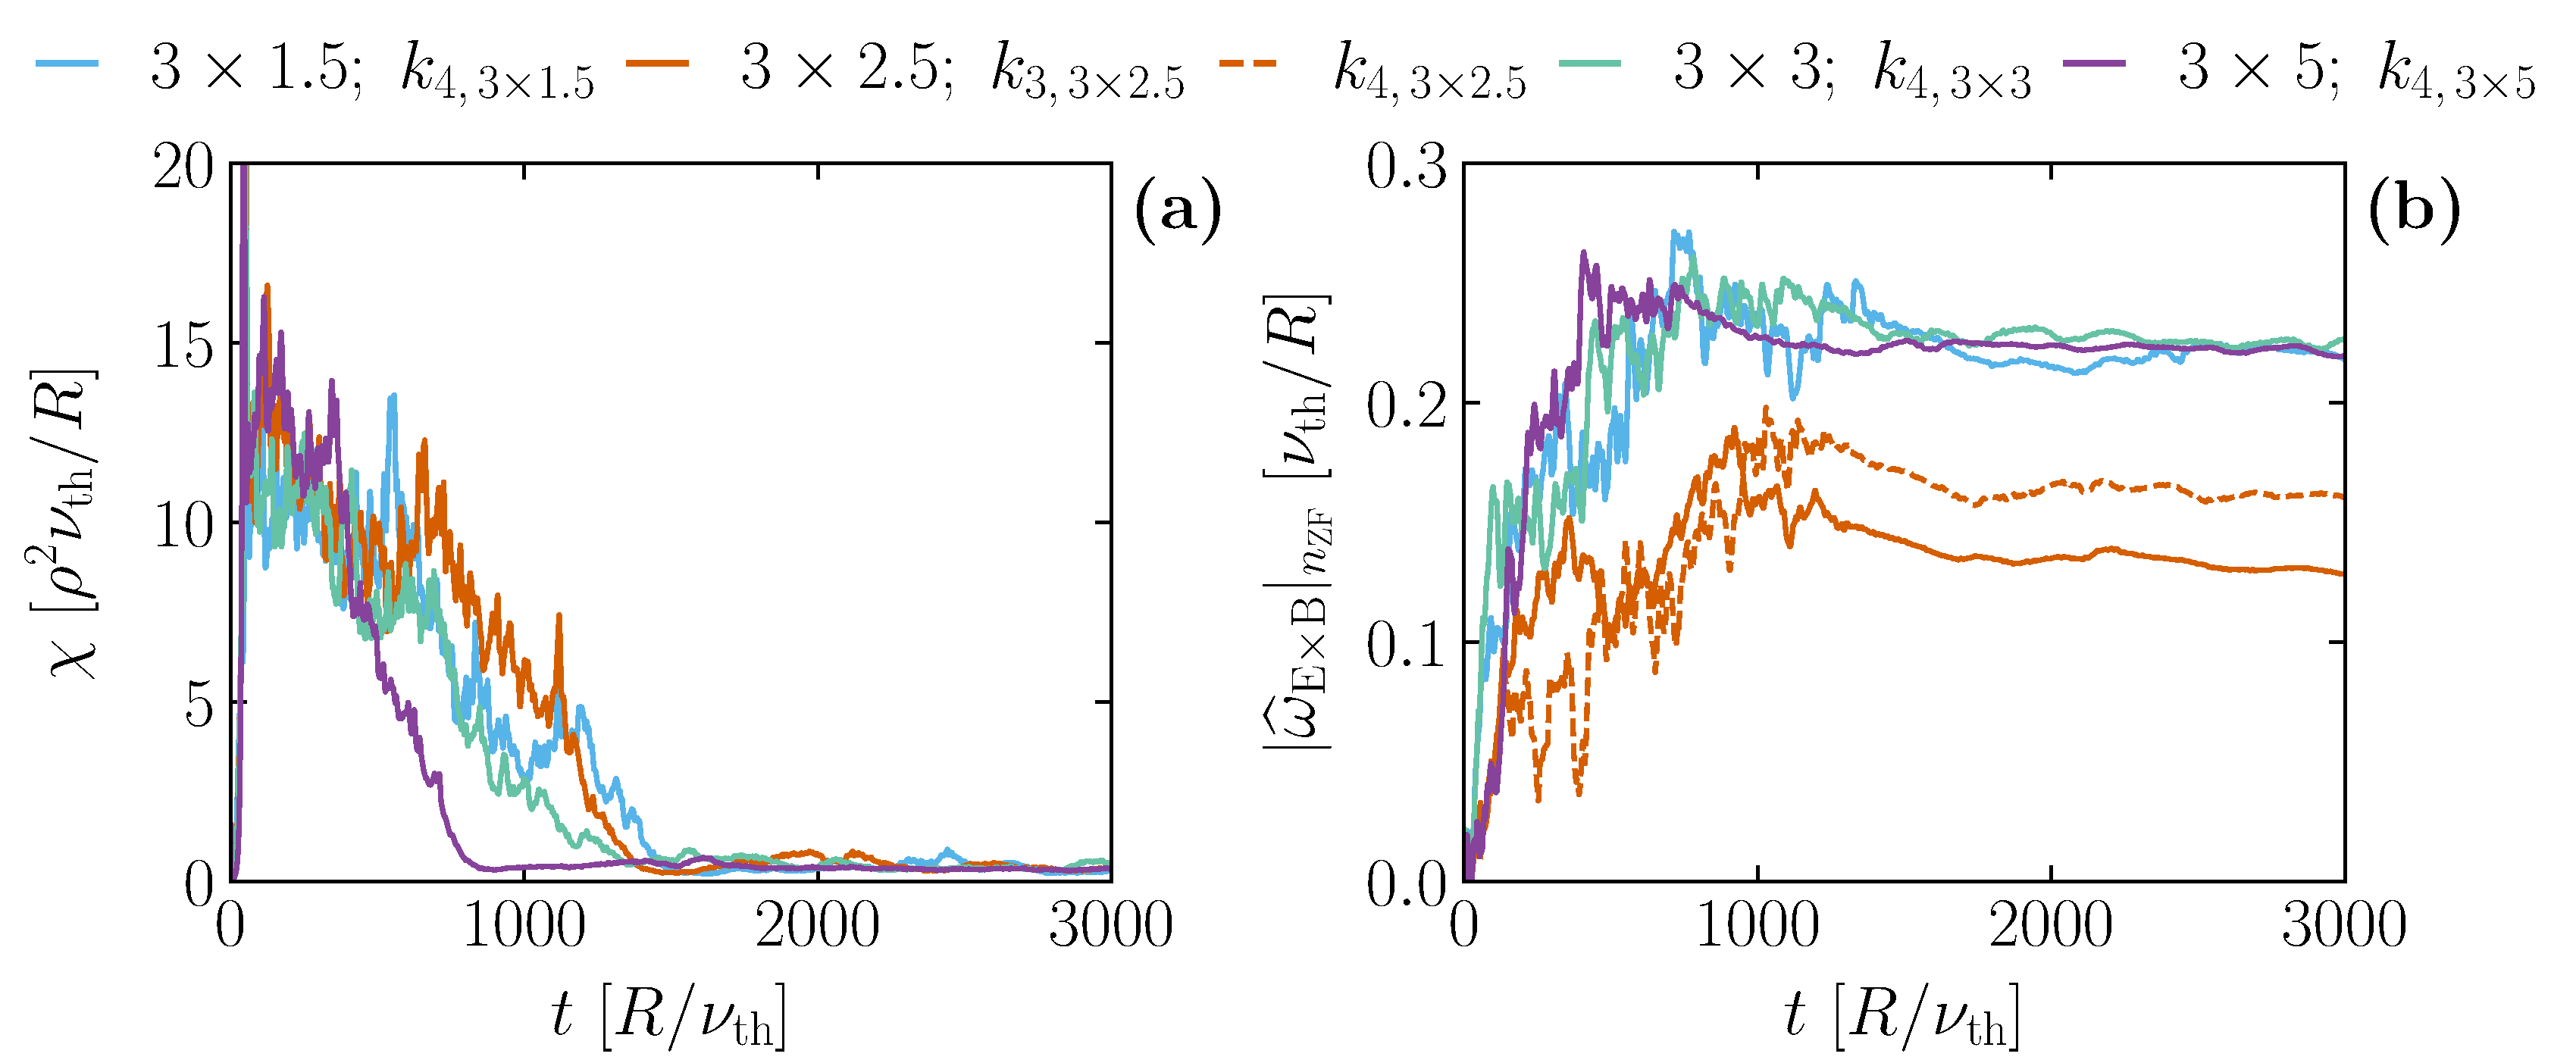
\includegraphics[width = 0.8\paperwidth]{Comparison/Boxsize/S6_rlt6.0_boxsize3x1-1.5-2.5-3-5_Ns16_Nvpar48_Nmu9_comparison_thesis.pdf}}
			
			\only<12>{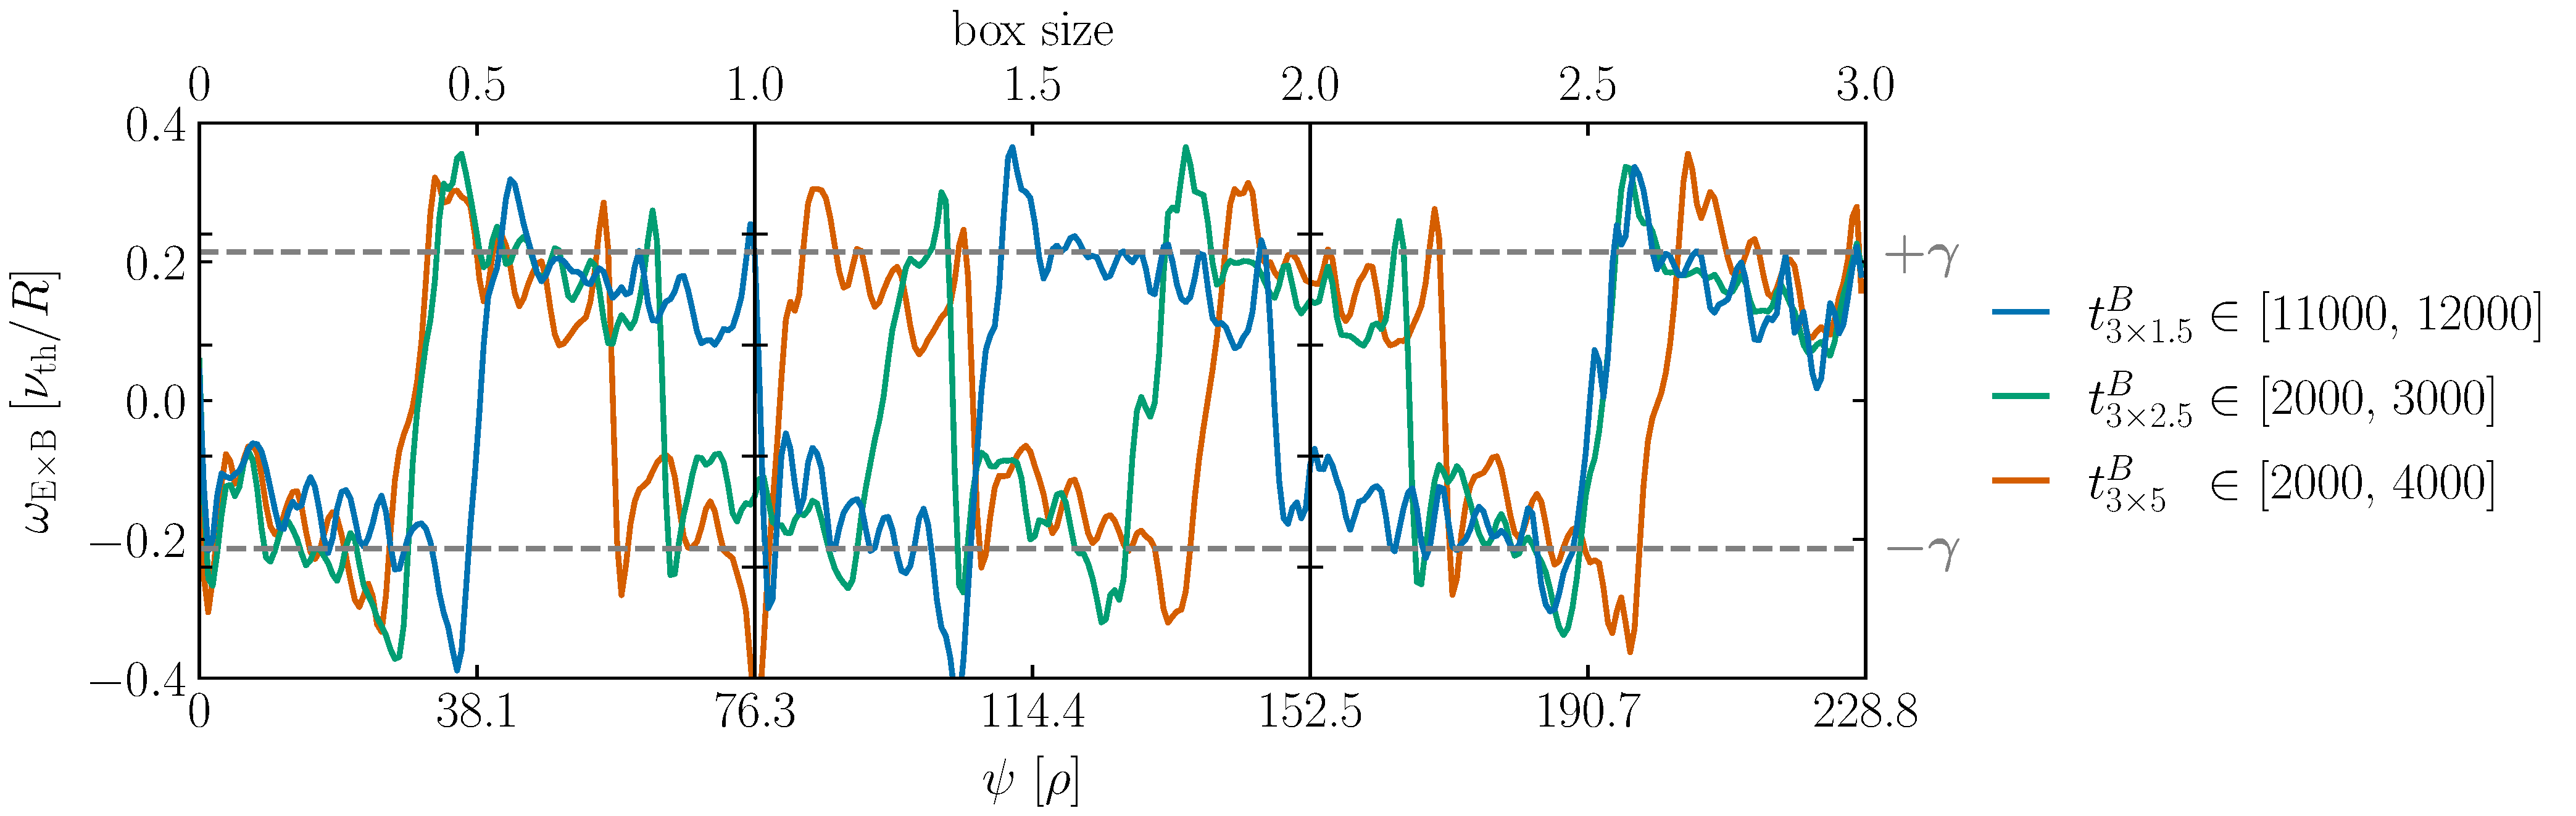
\includegraphics[height = 0.5\paperheight]{Comparison/Boxsize/S6_rlt6.0_boxsize3x1-1.5-2.5-3-5_Ns16_Nvpar48_Nmu9_wexb_comparison.pdf}}
		\end{center}

		\only<13>{
			\begin{center}
				$\Rightarrow$ Mesoscale pattern size of: \\[0.3cm]
				$\boxed{\sim 57 - 76\,\rhoth}$ \bigskip
				\begin{itemize}
					\item Non-locality is inherent to ITG-driven turbulence
					\item Avalanches are spatially organized by the E × B staircase pattern
				\end{itemize}
			\end{center}
		}
	\end{frame}

	\begin{frame}
		\frametitle{The finite Heat Flux Threshold}
		\begin{center}
			\onslide<2->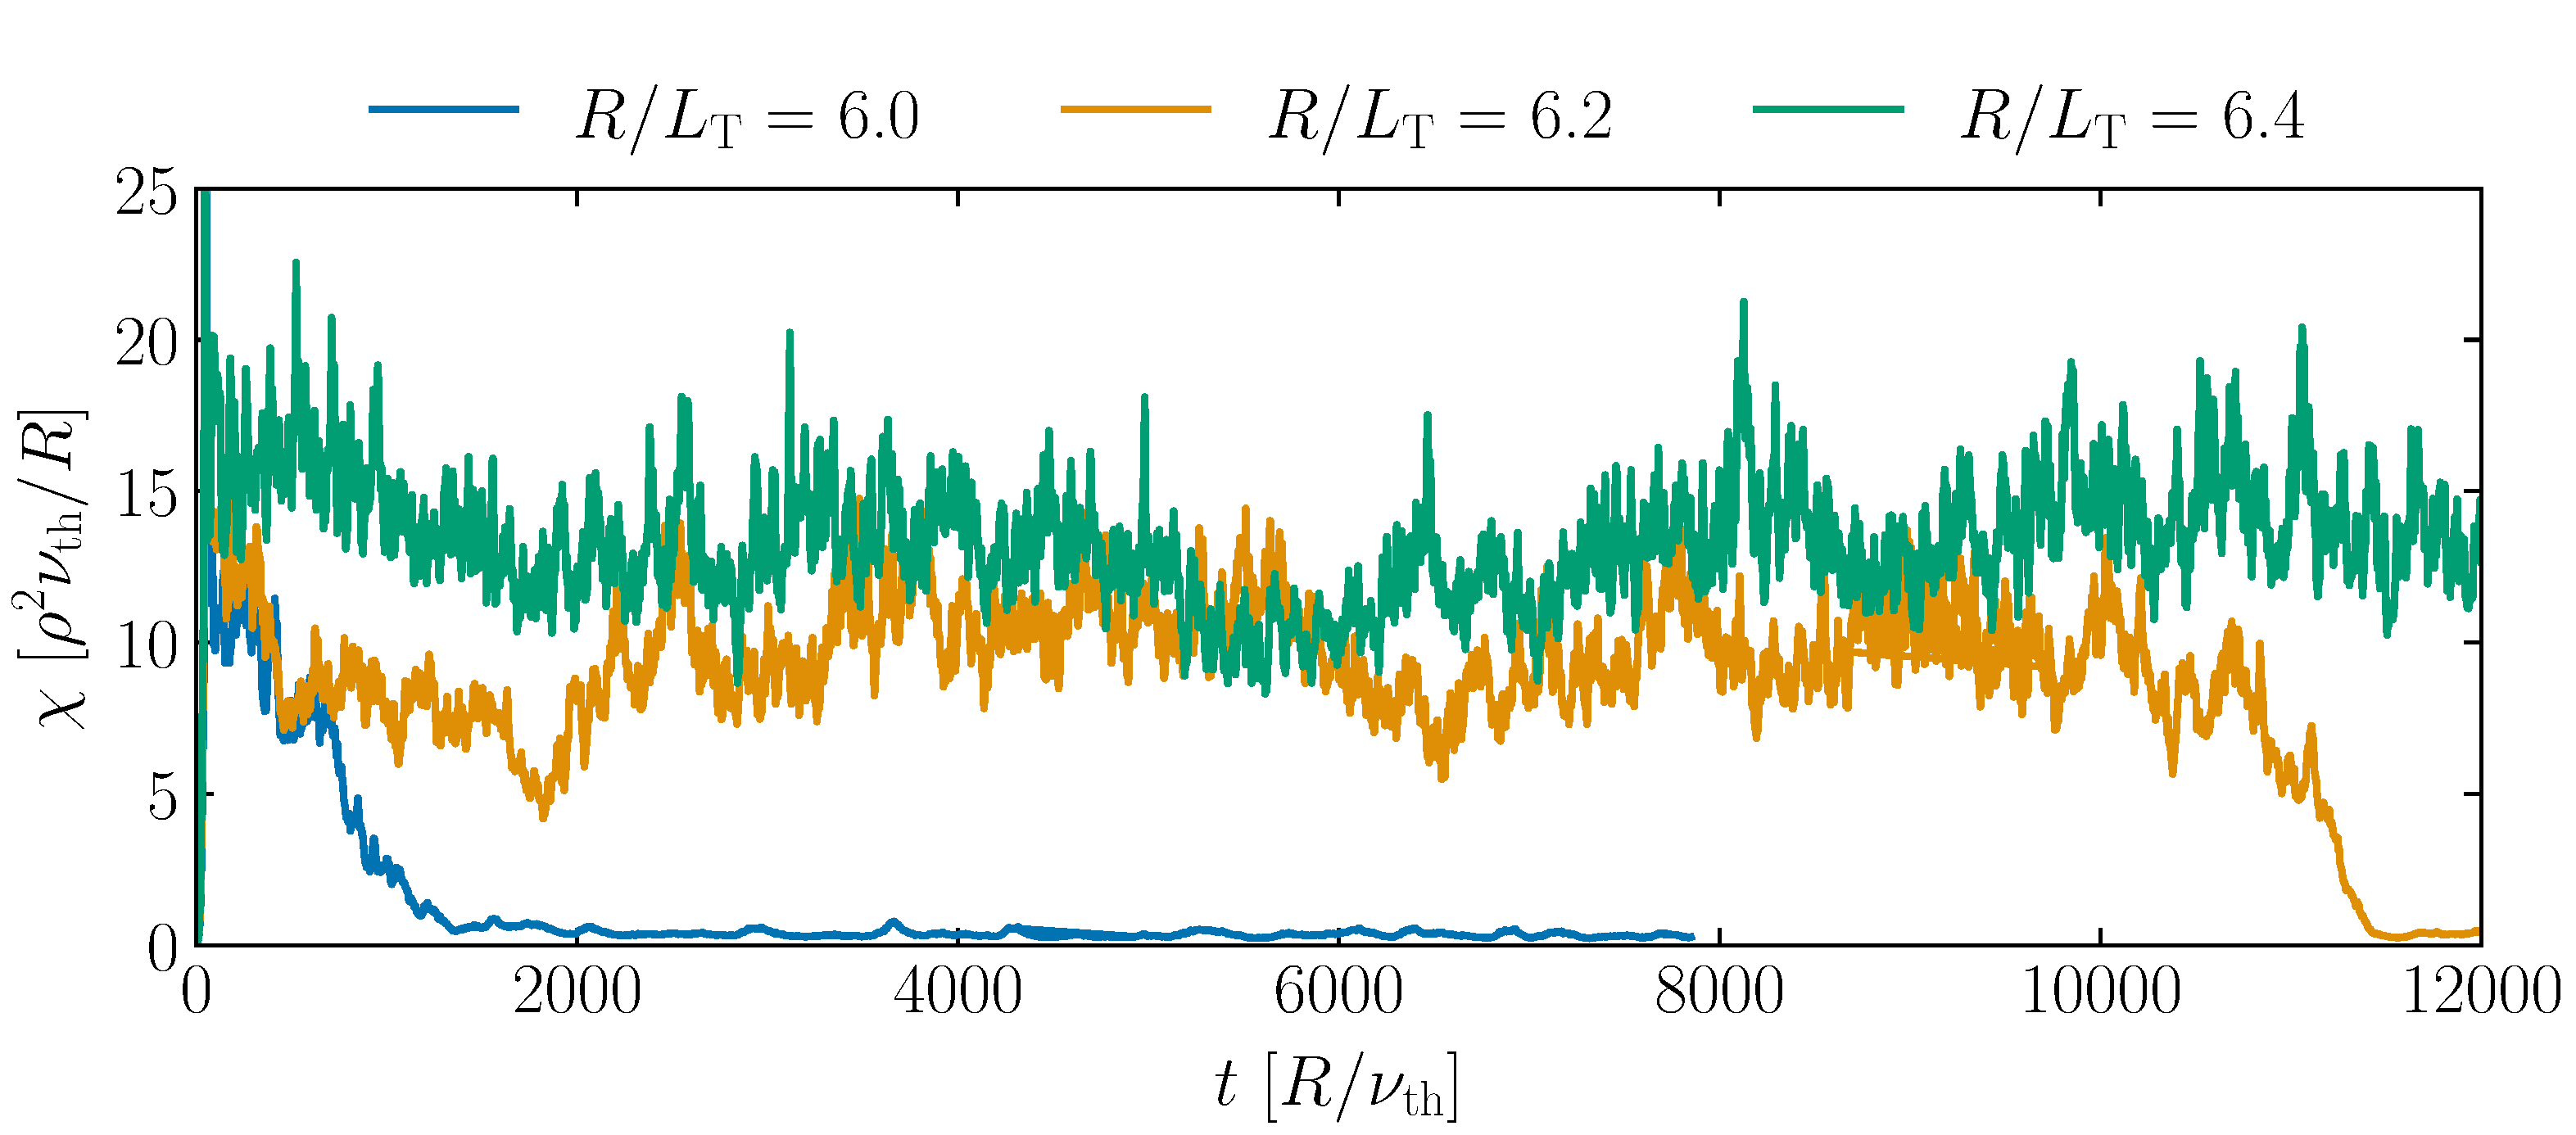
\includegraphics[width = 0.8\paperwidth]{Comparison/Gradient-Length/S6_rlt6.0-6.2-6.4_boxsize3x3_Ns16_Nvpar48_Nmu9_eflux_comparison.pdf}

			\onslide<3->$\Rightarrow~\boxed{\rlt|_\mathrm{finite} = 6.3 \pm 0.1}$
		\end{center}
	\end{frame}


	\section*{Conclusion}

	\begin{frame}
		\frametitle{Conclusion}
		
		\begin{minipage}{0.4\paperwidth}\raggedleft
			\begin{itemize}
				\item <2-> Parallel velocity $\Nvpar$ could be reduced from 64 to 48, which halfed the time until suppression of turbulence
				\item <3-> Restart Script with \texttt{python} led to further convenience during the task of performing simulations
				\item <4-> Mesoscale pattern size of $\sim 57 - 76\,\rhoth$ is found to be intrinsic to ITG-driven turbulence for Cyclone Base Case parameters
				\item <5-> Finite heat flux threshold is located at $\rlt|_\mathrm{finite} = 6.3 \pm 0.1$
			\end{itemize}
		\end{minipage}
		\begin{minipage}{0.4\paperwidth}
			\onslide<4-> 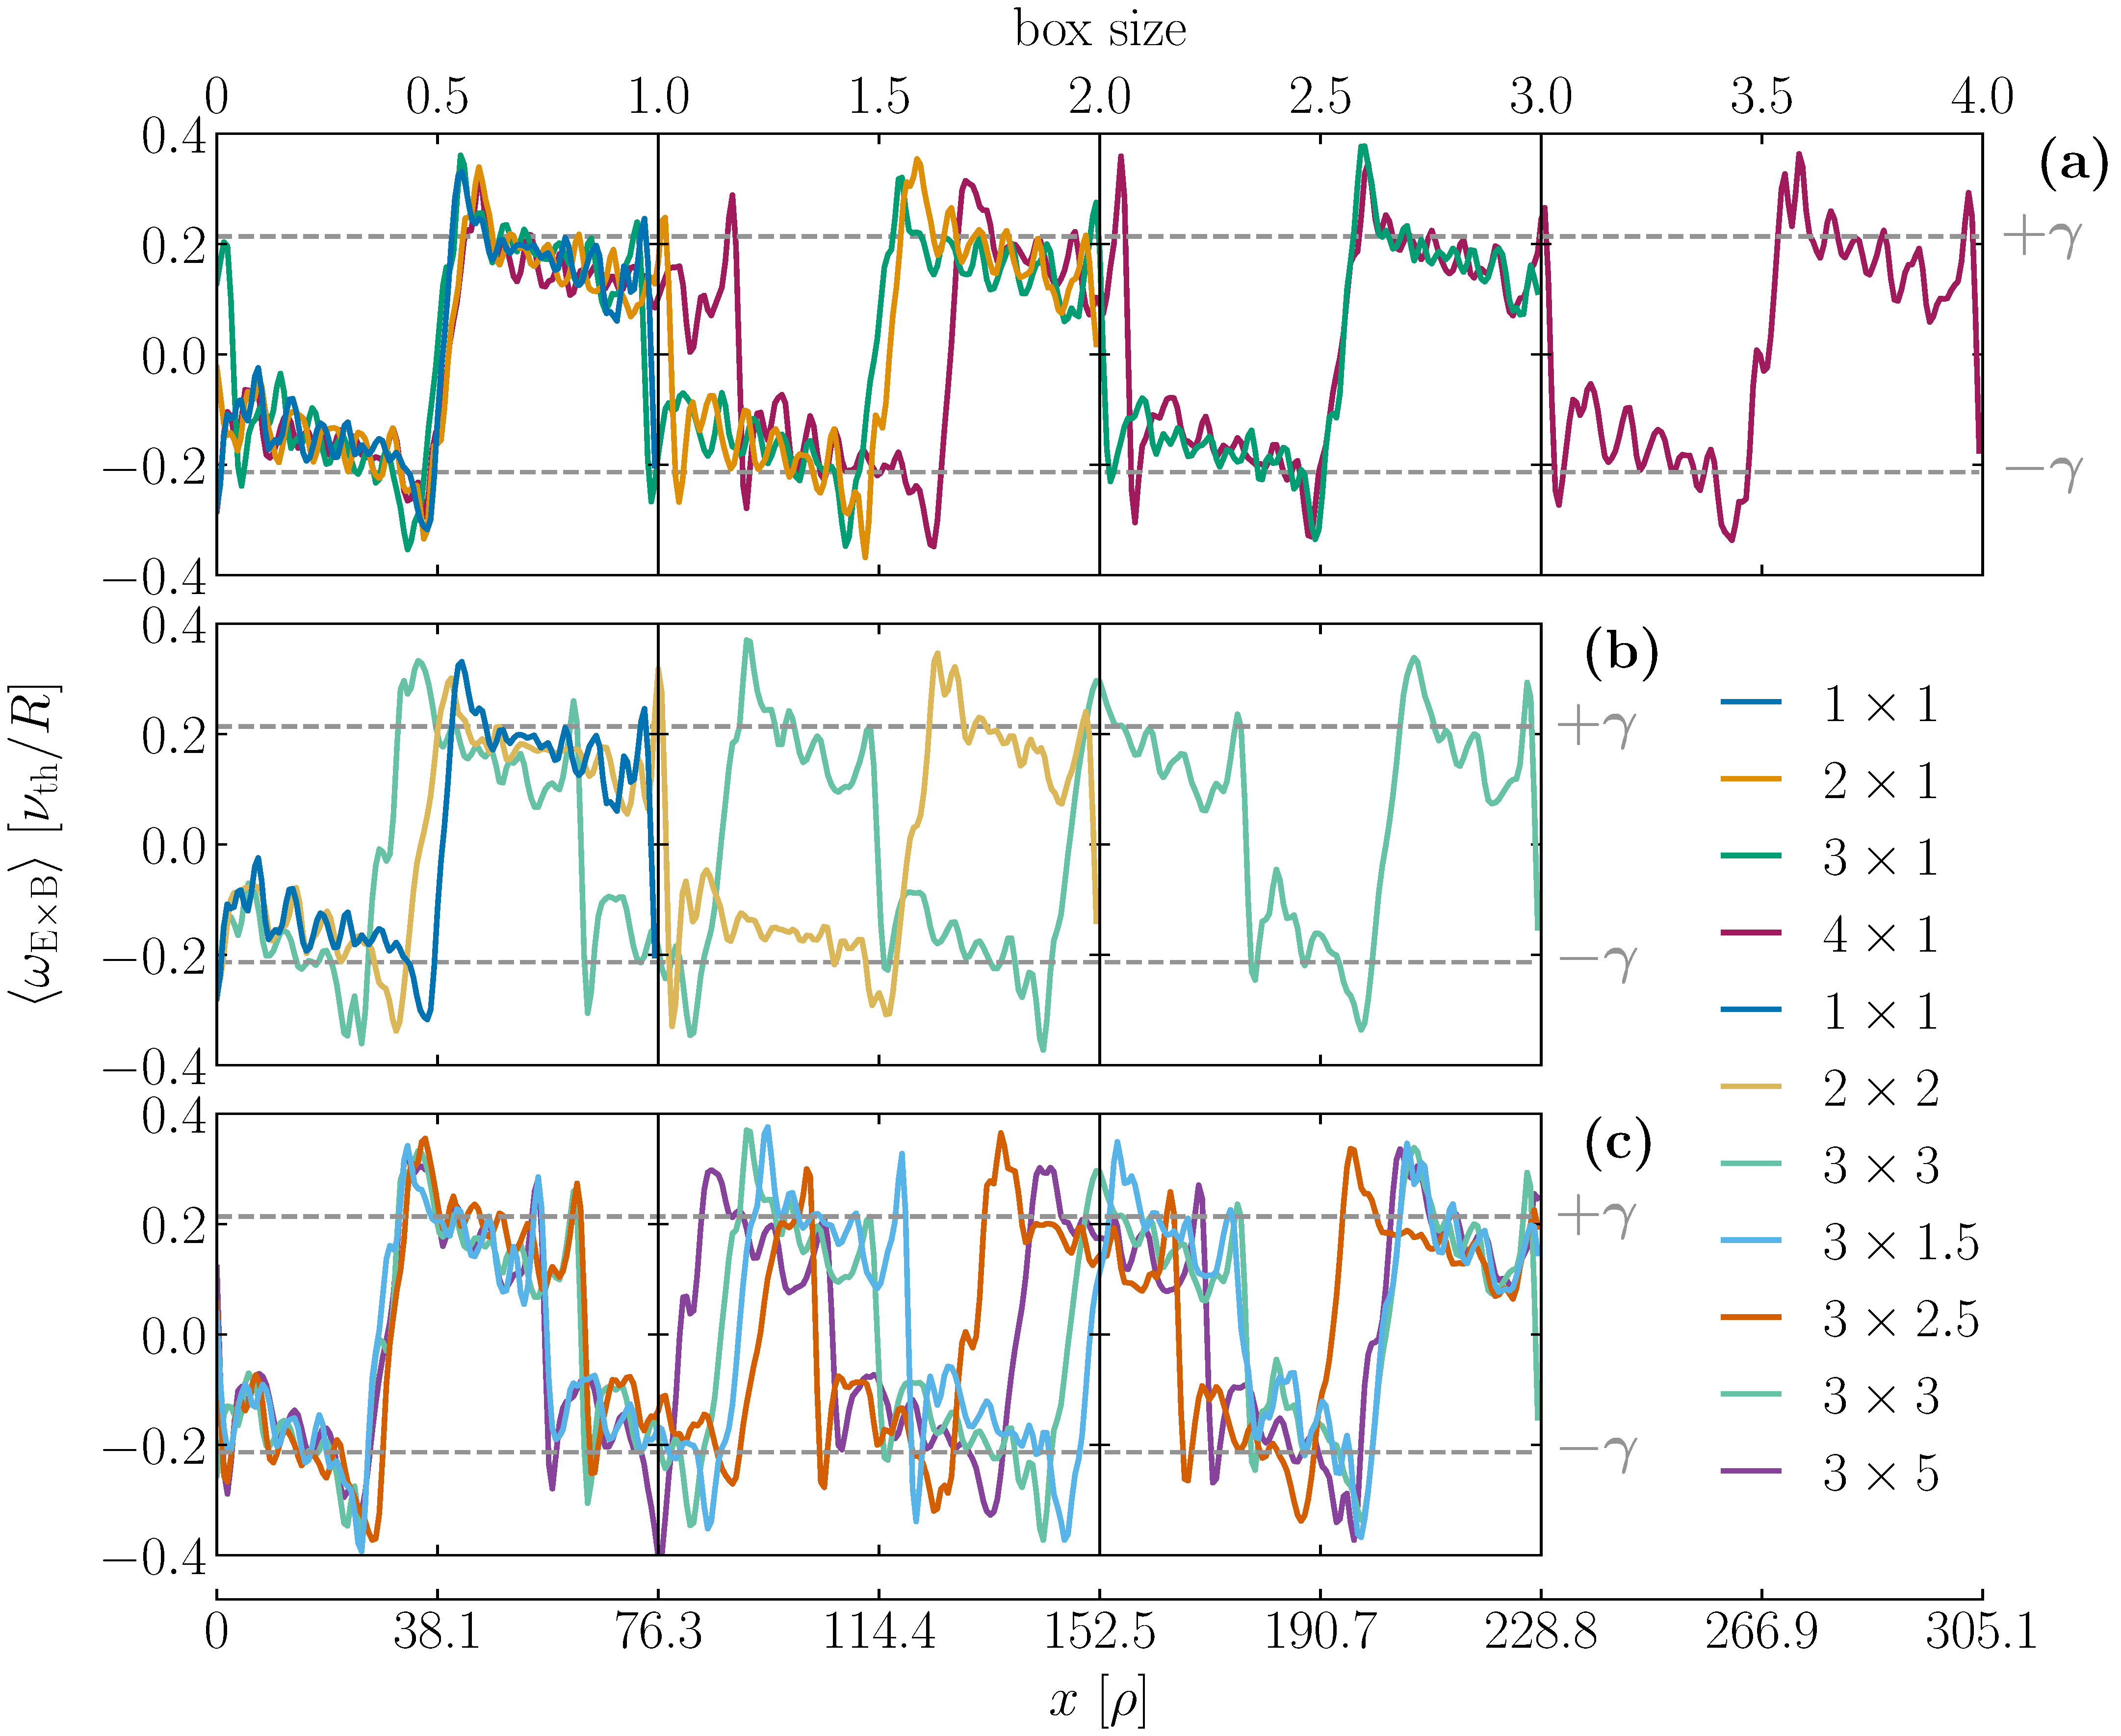
\includegraphics[width = 0.5\paperwidth]{Comparison/Boxsize/S6_rlt6.0_boxsize1-2-3-4x1-1.5-2-2.5-3-5_Ns16_Nvpar48_Nmu9_wexb_comparison_thesis.pdf}
		\end{minipage}
	\end{frame}

\end{document}






